\documentclass[12pt]{article}

\usepackage{booktabs}% http://ctan.org/pkg/booktabs
\usepackage[utf8]{inputenc}
\usepackage{changepage}
\usepackage{pgfplots}
\usepackage{amssymb}
\usepackage{xcolor}
\usepackage{hyperref}
\usepackage{listings}
\usepackage[T1]{fontenc}
\usepackage[utf8]{inputenc}
\usepackage{adjustbox}
\usepackage{amsmath}
\usepackage{mathtools}
\usepackage{biblatex}
\usepackage{float}
\usepackage{algorithm2e}
\lstset{
  language=Python,
  numbers=left,
  numberstyle=\tiny,
  stepnumber=1,
  numbersep=5pt,
  tabsize=4,
  basicstyle=\ttfamily,
  columns=fullflexible,
  keepspaces,
}
\hypersetup{
    colorlinks,
    citecolor=black,
    filecolor=black,
    linkcolor=black,
    urlcolor=black
}

% Set page size and margins
% Replace `letterpaper' with `a4paper' for UK/EU standard size
\usepackage[letterpaper,top=2cm,bottom=2cm,left=3cm,right=3cm,marginparwidth=1.75cm]{geometry}

% Useful packages
\usepackage{amsmath}
\usepackage{mathtools}
\usepackage{graphicx}
\newenvironment{para}{\begin{adjustwidth}{13mm}{}}{\end{adjustwidth}}

\newcommand\tab[1][1cm]{\hspace*{#1}}

\newcommand{\tabitem}{\llap{\textbullet}}
\newcommand{\Hsquare}{%
\text{\fboxsep=-.2pt\fbox{\rule{0pt}{1ex}\rule{1ex}{0pt}}}%
}

\newtheorem{Definizione}{Definizione}[subsection]
\newtheorem{Lemma}{Lemma}[subsection]
\newtheorem{Teorema/Definizione}{Teorema/Definizione}[subsection]
\newtheorem{Corollario}{Corollario}[subsection]
\newtheorem{Teorema}{Teorema}[subsection]
\newtheorem{Proposizione}{Proposizione}[subsection]
\newtheorem{Notazione}{Notazione}[subsection]
\newtheorem{Commento}{Commento}[subsection]
\newtheorem{Dimostrazione}{Dimostrazione}[subsection]
\newtheorem{Osservazione}{Osservazione}[subsection]
\newtheorem{Nota}{Nota}[subsection]

\title{RSO: Reti}
\author{spitfire}
\date{A.A. 2024-2025}
\begin{document}
\begin{figure}
    \centering
    
\includegraphics[width=0.35\textwidth]{Images/Logo scienze bicocca.png}
\end{figure}

\vspace{10cm}
\date{A.A. 2024-2025}


\maketitle

\newpage

\tableofcontents
\newpage
\section{Introduzione}
Se vogliamo dare una visione "d'insieme" di internet possiamo pensarlo come formato dalle
seguenti componenti:
\begin{itemize}
    \item Miliardi di \textbf{calcolatori} connessi:
    \begin{itemize}
        \item \textbf{Hosts}: dispositivi di computazione e sistemi periferici
        \item Sono sistemi che eseguono \textbf{applicazioni di rete} al "confine" della rete
    \end{itemize}
    \item \textbf{Packet switches}: inoltrano i pacchetti ("pezzi" di dati) tra diversi nodi di rete
    \begin{itemize}
        \item Router, switches, ...
        \item Internet è una \textbf{rete a commutazione di pacchetto}
    \end{itemize}
    \item \textbf{Communication links}: I collegamenti fra i veri nodi della rede
    \begin{itemize}
        \item Fibra, rame, radio, satellite...
        \item \textbf{Transmission rate}: capacità, in termini di bit/s, che il canale può supportare ("larghezza di banda").
    \end{itemize} 
    \item \textbf{Networks}: Collezioni di dispositivi, router, switches e links gestiti \textbf{tutti da una stessa organizzazione}
    \begin{itemize}
        \item Reti residenziali, enterprise ecc... vengono dette solitamente \textbf{reti di accesso}, perché sono quelle reti che raccolgono il traffico
        dagli utenti per mandarlo in rete o viceversa.
    \end{itemize}
\end{itemize}
\begin{center}
    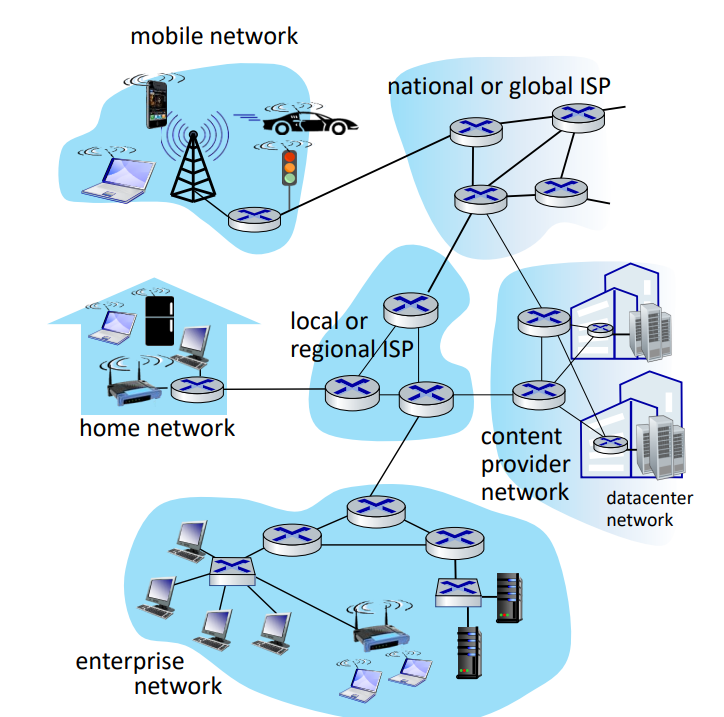
\includegraphics[width = 0.70\linewidth]{Images/1.PNG}
\end{center}
Internet è fisicamente una \textbf{rete connessa}, tuttavia vi sono dei sistemi che permettono di filtrare il traffico (firewall ecc...) per impedire che
ogni nodo della rete sia accessibile da un qualsiasi altro nodo. Internet è quindi una \textbf{rete di reti} che interconnette le reti
degli \textbf{Internet Service Providers} (ISP), cioè quelle entità che forniscono servizi di connettività. Il funzionamento della rete internet è governato
dai \textbf{protocolli di comunicazione}:
\begin{itemize}
    \item Controllano il modo in cui avviene l'invio e il ricevimento dei messaggi
    \item Esempi sono i protocolli HTTP (web), TCP, IP, WiFi, 4G, Ethernet ecc..
\end{itemize}
Protocolli di tipo diverso servono per \textbf{far comunicare dispositivi di tipo diverso}.
Poiché il contesto delle reti è quindi molto eterogeneo, il tutto riesce a funzionare grazie agli \textbf{standard}.
Esistono diversi enti di standardizzazione, tra cui citiamo:
\begin{itemize}
    \item \textbf{RFC}: Request for Comments, documenti
    \item \textbf{IETF}: Internet Engineering Task Force; rilascia le RFC
\end{itemize}
Il compito degli enti di standardizzazione è quello di rilasciare documenti che vanno a definire le caratteristiche
dei protocolli e delle architetture. Possiamo tuttavia vedere internet anche dal punto di vista dei \textbf{servizi}:
internet può essere quindi vista come una \textbf{infrastruttura che offre dei servizi di connettività alle applicazioni distribuite}.
Quindi, internet viene vista come una infrastruttura che \textbf{offre dei servizi di connettività tra nodi diversi}.
\begin{center}
    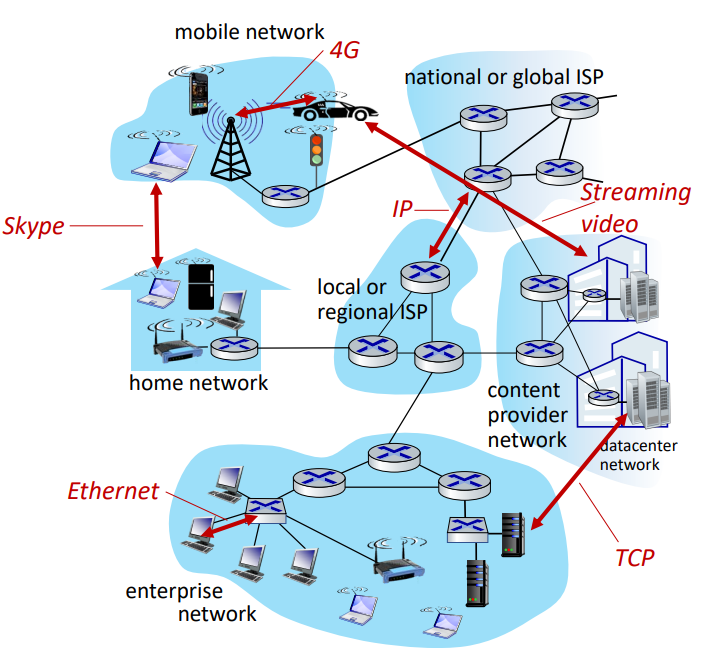
\includegraphics[width = 0.70\linewidth]{Images/2.PNG}
\end{center}
Abbiamo detto che la rete è governata da protocolli, ma \textbf{qual'è la definizione formale di protocollo?}
Una definizione formale può essere la seguente: i \textbf{protocolli} definiscono il \textbf{formato, l'ordine} dei \textbf{messaggi inviati e ricevuti} tra le entità di rete e le
\textbf{azioni intraprese} alla trasmissione e alla ricezione di un messaggio.
\begin{center}
    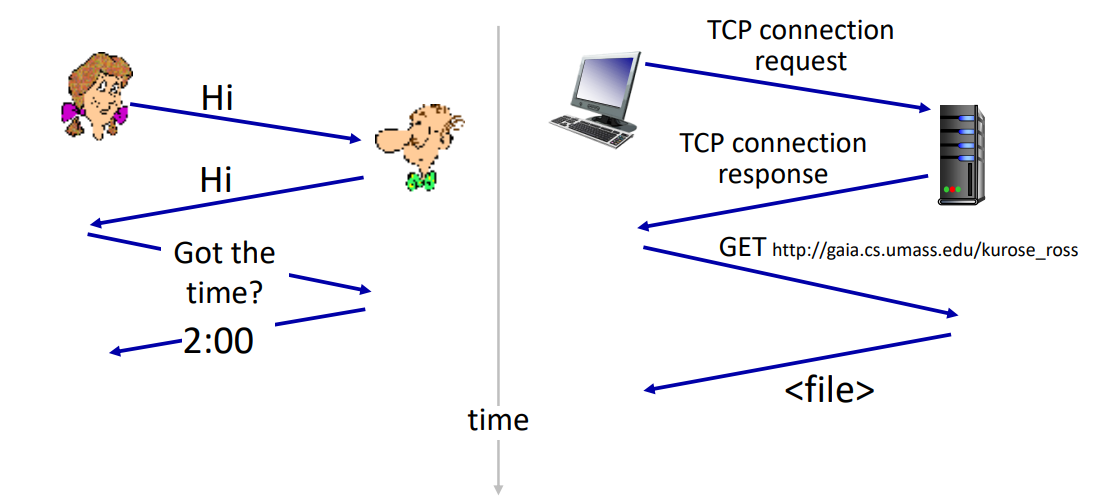
\includegraphics[width = 0.85\linewidth]{Images/3.PNG}
\end{center}
\subsection{Introduzione alla struttura di internet}
La struttura di alto livello di internet si può formalizzare nel seguente modo:
\begin{itemize}
    \item \textbf{Network edge}: il confine della rete, comprende
    \begin{itemize}
        \item \textbf{Hosts}: client e servers
        \item I servers sono spesso in \textbf{data centers}
    \end{itemize}
    È oggetto di dibattito se includere il confine della rete nella struttura di internet o meno; ciò nonostante, rimane comunque
    una componente fondamentale.
    \item \textbf{Access Networks}: Sono tutte quelle reti che servono a raccogliere il traffico generato e destinato per gli utenti.
    Sono quindi i \textbf{punti di accesso alla rete per gli utenti}. Esse possono essere \textbf{cablate oppure wireless}.
    \item \textbf{Network Core}: È l'insieme di tutte quelle reti che sono composte da router interconnessi che permettono di realizzare il concetto di \textbf{rete di reti}.
    Il suo compito è quello di \textbf{connettere le reti di accesso fra di loro} e comprendono tutte quelle reti che, su larga scala, \textbf{permettono il funzionamento di internet}.
\end{itemize}
Ogni componente della struttura di internet viene detto \textbf{segmento}.
\subsubsection{Network Edge}
Il confine della rete è \textbf{popolato dagli host}. Il suo compito principale è quello di inviare i \textbf{pacchetti}
generati dagli host (e quindi dagli utenti). Una visione ad alto livello di questo procedimento è:
\begin{itemize}
    \item Il \textbf{messaggio applicativo} viene generato dall'host
    \item Esso viene \textbf{spezzettato in pezzetti}, chiamati \textbf{pacchetti}, di lunghezza $L$ bits (questa cosa non è sempre vera: ci sono casi in cui i pacchetti hanno lunghezza variabile).
    Ognuno di questi pacchetti presenta una \textbf{intestazione}, cioè un determinato numero di bit che servono per permettere il funzionamento dei protocolli in rete
    \item Una volta generati i pacchetti, essi vengono trasmessi alla rete d'accesso ad un \textbf{tasso di trasmissione} (transmission rate) $R$, il quale è condizionato dalla \textbf{capacità di trasmissione del collegamento}
\end{itemize}
\begin{center}
    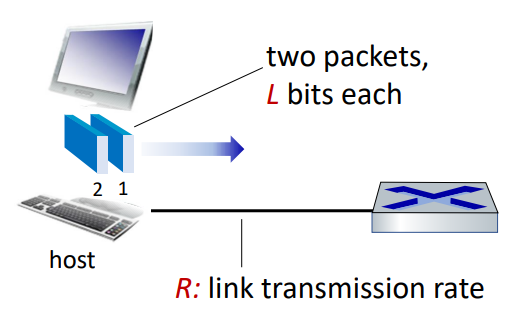
\includegraphics[width = 0.50\linewidth]{Images/4.PNG}
\end{center}
Ogni volta che invio un pacchetto in rete, ho un \textbf{ritardo di trasmissione}, il quale è il tempo necessario per trasmettere un pacchetto di $L$ bit su un collegamento che
ha capacità di trasporto di $R$ bit/sec. Quindi:
$$\textrm{packet transmission delay} = \frac{L \; (bits)}{R \; (bits/sec)}$$
\subsubsection{Access Networks}
Come facciamo a \textbf{connettere gli host a "internet"}? Il compito di effettuare questa connessione è delle
reti di accesso. Esse possono essere:
\begin{itemize}
    \item Reti di accesso \textbf{residenziali}
    \item Reti di accesso \textbf{istituzionali}
    \item Reti di accesso \textbf{mobili}
\end{itemize}
\subsubsection{Network Core}
La Network Core è un insieme di \textbf{maglie di rete interconnesse}, le quali sono fondamentali per effettuare le
operazioni di commutazione dei pacchetti. Esse garantiscono che i pacchetti possano essere trasmessi da un router verso l'altro
attraverso dei collegamenti da una sorgente a una destinazione.
Le reti di core presentano due \textbf{funzionalità fondamentali}:
per spiegarle, dobbiamo prima capire \textbf{come funziona un router}: esso possiede al suo interno una tabella chiamata
\textbf{tabella di inoltro} (forwarding table), che indica verso quale collegamento un pacchetto deve essere instradato in base al valore
della sua intestazione (che quindi contiene, in termini generici, a chi deve essere recapitato questo pacchetto).
L'operazione di \textbf{inoltro} (o \textbf{commutazione di pacchetto}) quindi consiste nell'invio sulla connessione corretta del pacchetto in arrivo (questa operazione viene anche detta \textbf{switching}).
L'inoltro ha \textbf{valenza locale}: ogni router prende in considerazione solo la propria tabella di inoltro locale per decidere dove inoltrare un pacchetto.
Tuttavia, questa operazione non basta per garantire che io possa raggiungere la destinazione corretta; per garantirlo dobbiamo effettuare un'altra operazione che prende il nome di
\textbf{instradamento} (routing). Il routing è un'operazione \textbf{globale} che è utilizzata per determinare \textbf{quale percorso, fra sorgente e destinazione, devono attraversare i pacchetti}.
Ogni singolo router esegui quindi dei \textbf{protocolli} e degli \textbf{algoritmi di routing distribuiti} che hanno l'obbietto di \textbf{popolare le tabelle di inoltro} (viene effettuato tramite algoritmi su grafo).
Poiché gli algoritmi di routing sono \textbf{distribuiti}, essi richiedono lo \textbf{scambio di messaggi e la collaborazione tra i router}.
\begin{center}
    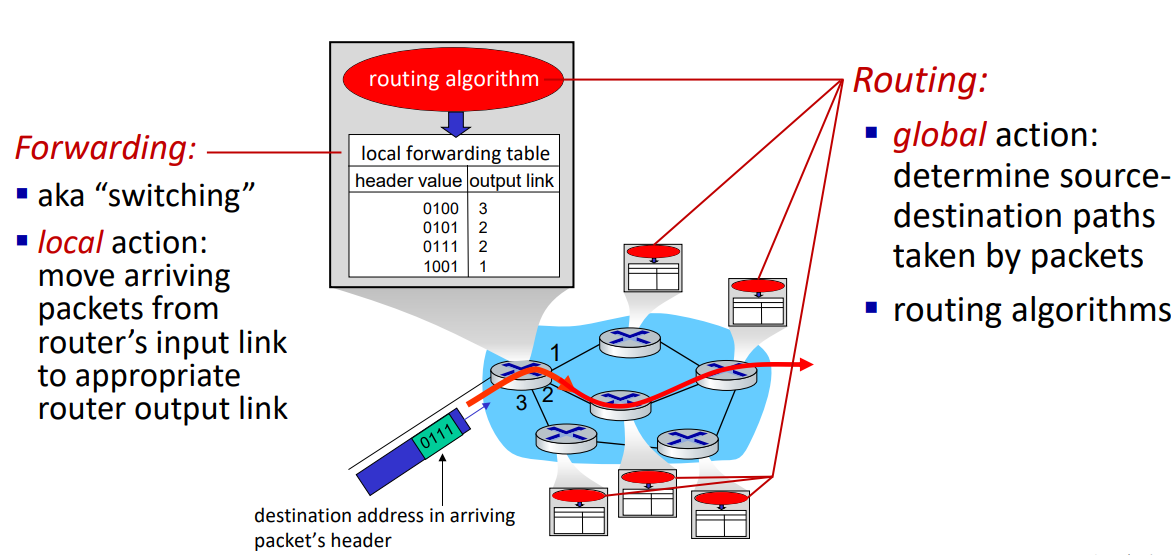
\includegraphics[width = 1\linewidth]{Images/5.PNG}
\end{center}
\subsection{Packet Switching: Store-and-Forward}
Nelle reti a commutazione di pacchetto, \textbf{ogni pacchetto ha vita propria}: una volta che il messaggio viene spezzettato in pacchetti, ognuno di esso
ha un ciclo di vita indipendente dagli altri. La modalità di trasmissione usata da tutte le reti a commutazione di pacchetto è quella del \textbf{store-and-forward}:
quando un pacchetto arriva ad un commutatore per essere commutato, esso deve \textbf{arrivate interamente prima di essere trasmesso al nodo successivo}. Tuttavia, si può pensare
di saltare questo passaggio e trasmettere direttamente ogni bit che arriva su un certo nodo al successivo. Perché non viene fatto nelle reti a commutazione di pacchetto? Il motivo risiede nelle \textbf{intestazioni dei pacchetti}:
infatti, è li che trovo \textbf{tutte le informazioni necessarie per gestire un pacchetto}, quindi devo aspettare che essa venga trasmessa per intero prima di procedere all'invio al nodo successivo.
\begin{center}
    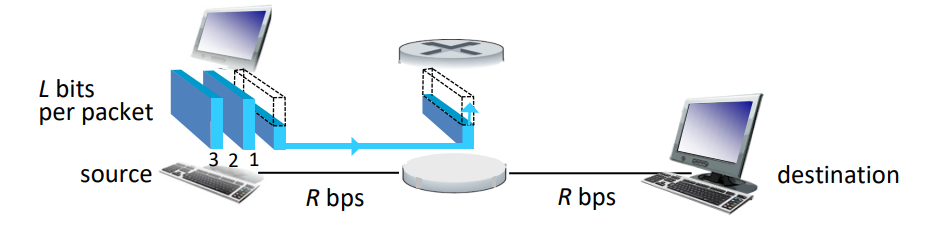
\includegraphics[width =1\linewidth]{Images/6.PNG}
\end{center}
\subsection{Packet-Switching: queuing}
Seppur Store-and-Forward semplifichi di molto la gestione delle reti, esso introduce una problematica che prende il nome di
\textbf{accodamento} (queueing). È una problematica che esiste in tutte le reti e si manifesta quando il \textbf{tasso di arrivo dei pacchetti è superiore al tasso di trasmissione in uscita}.
Nei router e negli switch, i pacchetti si accodano in aree di memoria apposite dette \textbf{buffer}; un pacchetto rimane nel buffer fino a quando non verrà trasmesso.
\begin{center}
    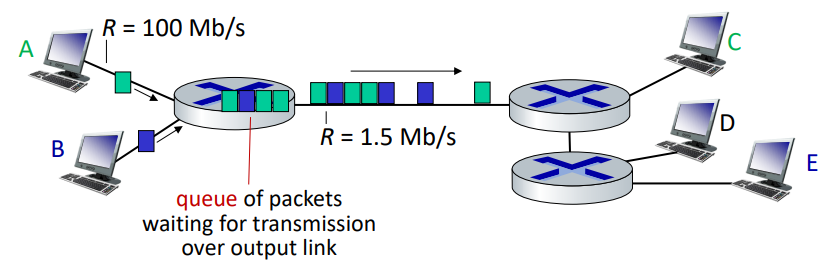
\includegraphics[width =0.90\linewidth]{Images/7.PNG}
\end{center}
Questa è una condizione che può accadere nelle reti a commutazione di pacchetto, tuttavia \textbf{non può essere una situazione sistematica}:
se si verificasse costantemente, la dimensione del buffer \textbf{crescerebbe costantemente} fino a raggiungere la massima dimensione possibile; da quel momento
in poi ogni pacchetto in arrivo porta a una condizione di \textbf{buffer overflow} e andrebbe perso. Quindi, quali sono i problemi che provoca l'accodamento?
\begin{itemize}
    \item \textbf{Buffer overflow} dei buffer dove vengono salvati i pacchetti ancora da trasmettere e susseguente perdita dei pacchetti in arrivo
    \item \textbf{Ritardo di accodamento} dato dall'attesa che il router trasmetta il pacchetto
\end{itemize}
\subsection{Circuit Switching}
La commutazione di pacchetto non è l'unico tipo di commutazione esistente; anzi essa storicamente è posteriore ad un'altro tipo di commutazione
che prende il nome di \textbf{commutazione a circuito}
\begin{center}
    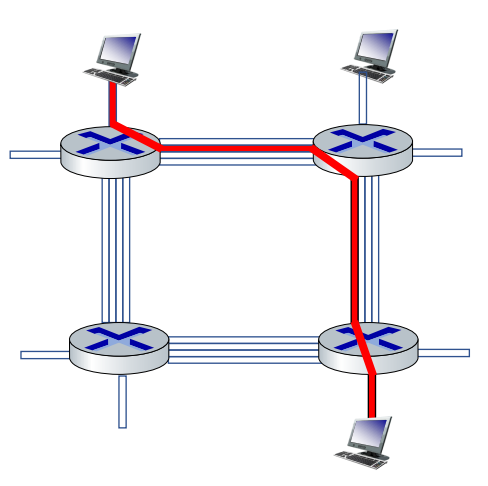
\includegraphics[width =0.45\linewidth]{Images/8.PNG}
\end{center}
Questo tipo di commutazione segue un principio diverso da quella a commutazione di pacchetto: l'elemento fondamentale di questo tipo di rete è il \textbf{circuito} (non esistono i pacchetti in questo tipo di rete).
Tra i vari \textbf{commutatori di circuito} si possono stabilire un certo numero di circuiti.
L'obbiettivo di questo tipo di commutazione è \textbf{destinare i circuiti alla comunicazione tra gli utenti della rete}.
Le risorse di un circuito vengono \textbf{assegnate in maniera esclusiva ad un host} e non possono essere condivise con altri host.
Il vantaggio di questo tipo di commutazione è \textbf{l'assenza di accodamento} data dal completo assegnamento delle risorse di un circuito
ad una sola comunicazione tra sorgente e destinazione.
Viene chiamato \textbf{circuito end-to-end} l'insieme di tutti i circuiti che vengono stabiliti tra sorgente e destinazione.
Uno svantaggio di questo tipo di commutazione è la \textbf{necessità di una fase di setup} in cui vengono allocate le risorse dei circuiti per andare a creare
il circuito end-to-end.
\subsubsection{Packet Switching vs Circuit Switching}
In una commutazione di circuito, le risorse vengono allocate solamente alla comunicazione tra sorgente e destinazione e non esistono
problemi di accodamento. Tuttavia, l'utilizzo delle risorse di rete in questo tipo di comunicazione risulta \textbf{subottimale} rispetto ad una
rete a commutazione di pacchetto. Facciamo un esempio:
\begin{center}
    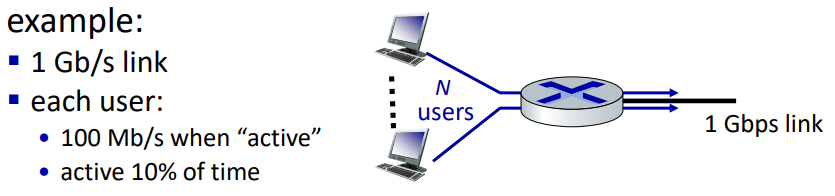
\includegraphics[width =0.75\linewidth]{Images/9.PNG}
\end{center}
\textbf{Domanda: quanti utenti, in queste condizioni, possono rispettivamente accomodare una rete a commutazione di circuito e una rete a commutazione di pacchetto?}
\begin{itemize}
    \item \textbf{Circuit-switching}: 10 utenti
    \item \textbf{Packet-switching}: con 35 utenti, la probabilità che più di 10 utenti siano attivi allo stesso tempo è minore di $0.0004$
\end{itemize}
Quindi una rete a commutazione di pacchetto è sempre la scelta migliore?
\begin{itemize}
    \item Essa è ottima per un traffico di tipo \textbf{"bursty"} (a raffica), cioè in situazioni dove a volte ci sono dati da inviare, a volte no
    \item Permette la condivisione delle risorse di rete
    \item Non richiede setup
\end{itemize}
Tuttavia, se si creano condizioni sfavorevoli, si vanno a creare delle \textbf{situazione di congestione eccessiva della rete}, andando a creare situazioni
di ritardo nella trasmissione dei pacchetti e di buffer overflow. Si rendono quindi necessari \textbf{protocolli di trasmissione affidabili} e meccanismi di \textbf{controllo della congestione}.
È però possibile, visti i vantaggi delle reti a commutazione di circuito, fornire lo stesso tipo di garanzia del servizio anche nelle reti a commutazione di pacchetto?
La risposta è si; esistono delle tecniche che permettono di \textbf{emulare la commutazione di circuito sulle reti a commutazione di pacchetto}, tuttavia sono casi parecchio difficili da gestire.
\subsection{Struttura di internet nel dettaglio}
Gli host sono connessi a internet tramite le \textbf{reti di accesso} fornite da ISPs.
Le reti di accesso devono per forza essere \textbf{interconnesse} per garantire che possa avvenire la comunicazione tra qualsiasi due host della rete (internet è una rete \textbf{connessa}, cioè ogni nodo è raggiungibile da tutti gli altri nodi).
Il risultato dell'evoluzione di internet è una \textbf{struttura gerarchica}; questa evoluzione, tuttavia, non è stata guidata da \textbf{necessità di tipo tecnico} ma di tipo \textbf{economico e politico}.
Vediamo quindi la struttura di internet passo passo: al mondo abbiamo \textbf{milioni} di reti di accesso
\begin{center}
    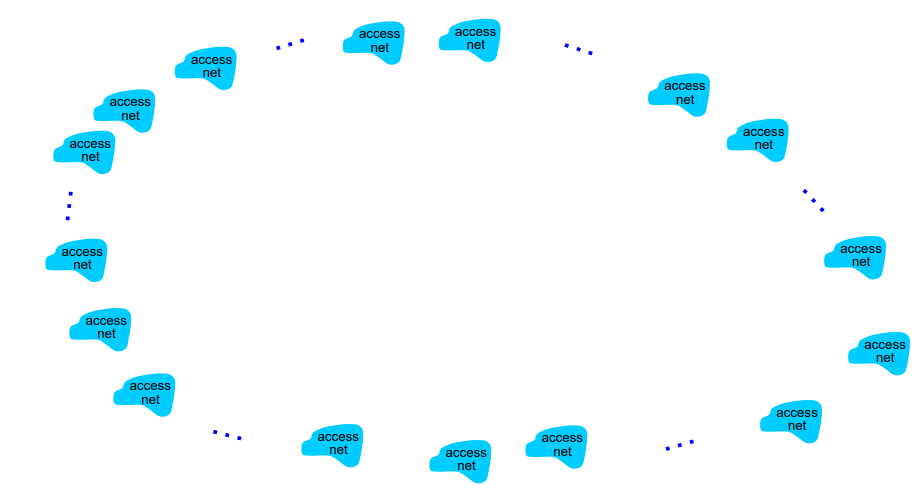
\includegraphics[width =0.85\linewidth]{Images/10.PNG}
\end{center}
L'idea più semplice per interconnetterle è \textbf{connettere ogni ISP agli altri in maniera diretta}, tuttavia...
\begin{center}
    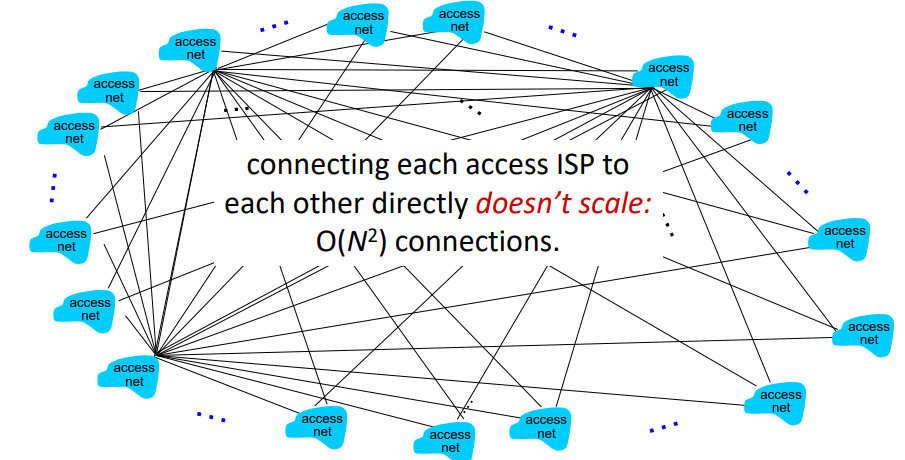
\includegraphics[width =0.85\linewidth]{Images/11.PNG}
\end{center}
Una soluzione alternativa è quella di avere un \textbf{ISP globale} (o di transito) con una rete geograficamente estesa in tutto il mondo, i cui router sono \textbf{interconnessi} e che fornisce connettività alle reti di accesso:
\begin{center}
    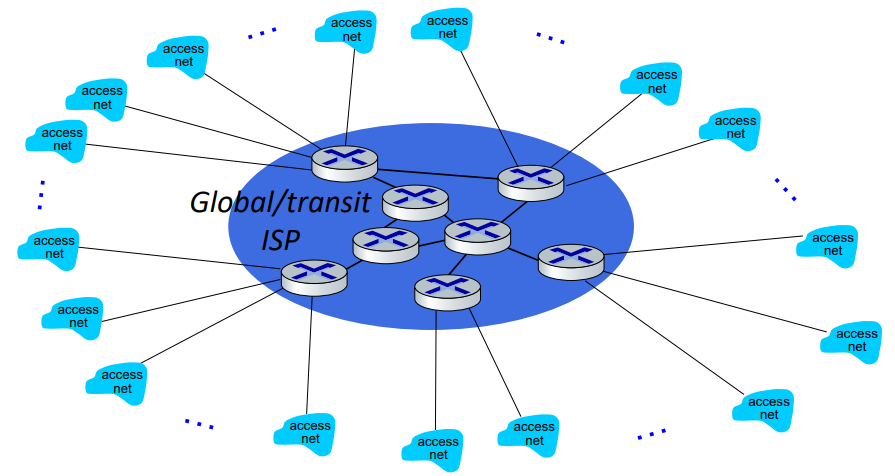
\includegraphics[width =0.85\linewidth]{Images/12.PNG}
\end{center}
Questo approccio tuttavia ha dei problemi:
\begin{itemize}
    \item Richiede una rete estesa \textbf{su tutto il globo}, in modo che possa servire ogni rete di accesso
    \item Richiede un accordo economico tra gli ISP locali e quello globale
    \item Perché ci si dovrebbe limitare ad un solo ISP globale? In effetti, ci potrebbe essere concorrenza fra essi
\end{itemize}
In virtù dell'ultimo punto sopra, si è andata a creare una situazione di questo tipo:
\begin{center}
    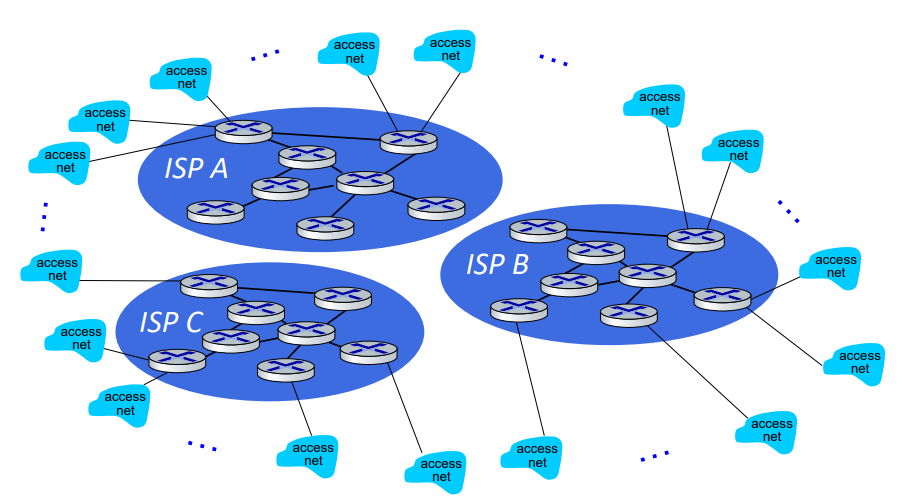
\includegraphics[width =0.85\linewidth]{Images/13.PNG}
\end{center}
si sono andati quindi a creare degli ISPs \textbf{geograficamente estesi} che coprono determinate aree del globo.
Questo genere di ISPs prendono il nome di \textbf{Tier 1 ISPs}.
A questo punto, gli ISPs globali devono creare dei \textbf{peering links} (chiamati così perché \textbf{non sono il frutto di un accordo economico ma di un accordo tra pari})
per creare un'interconnessione tra di loro:
\begin{center}
    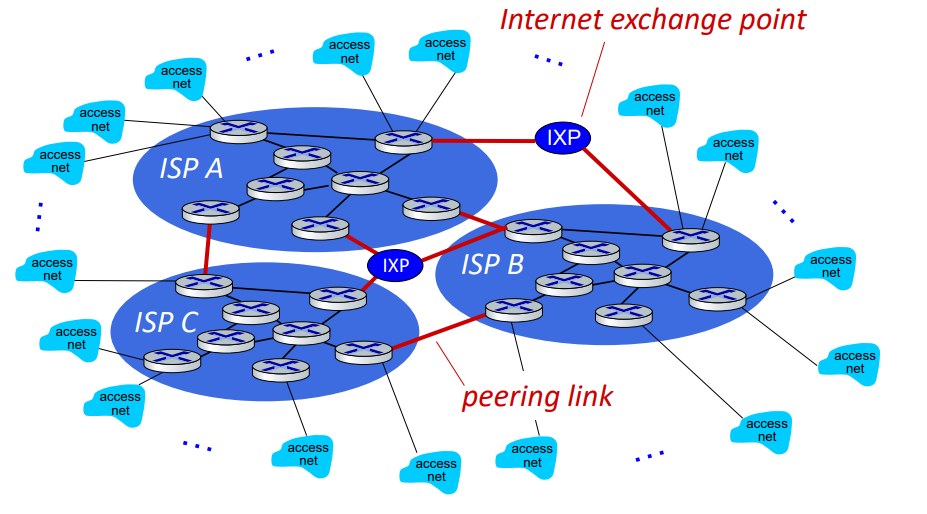
\includegraphics[width =0.85\linewidth]{Images/14.PNG}
\end{center}
Tuttavia, c'è anche un'altra possibilità, cioè quella di avere degli \textbf{Internet Exchange Points} (IXPs), i quali sono dei nodi a cui gli ISPs globali si connettono e che garantiscono
la connessione tra di essi. Tuttavia, tipicamente le reti di acceso non si \textbf{interfacciano direttamente con gli ISPs globali} ma passano tramite \textbf{ISPs regionali}, che hanno una diffusione
più capillare sul territorio. Altro tipo modo in cui le reti di accesso accedono agli ISPs globali è tramite \textbf{multi-homing}, cioè una rete di accesso potrebbe avere \textbf{più collegamenti verso un ISPs globale o regionale};
questo approccio garantisce \textbf{resilienza}
\begin{center}
    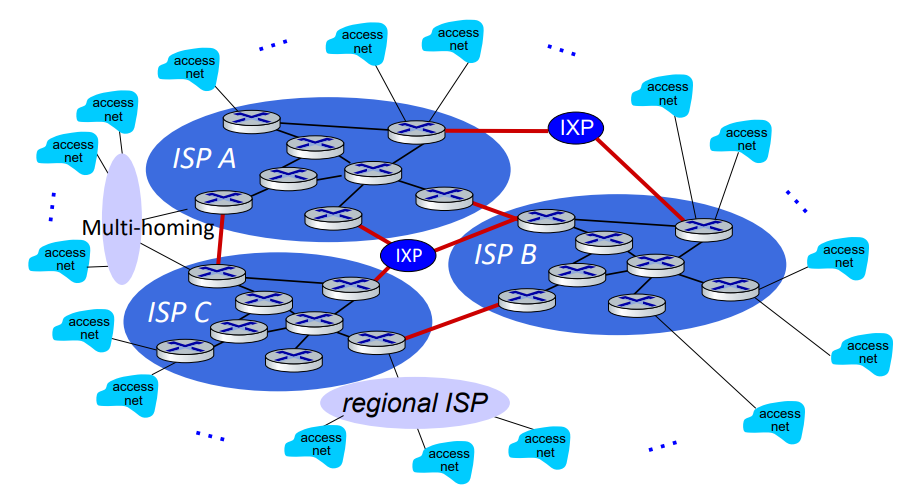
\includegraphics[width =0.85\linewidth]{Images/15.PNG}
\end{center}
Infine, abbiamo le \textbf{reti dei content provider}, che hanno lo scopo di \textbf{fornire contenuto agli utenti}. Per farlo, molto spesso, esse \textbf{bypassano gli ISPs globali} e si interfacciano
direttamente con le reti di accesso.
\begin{center}
    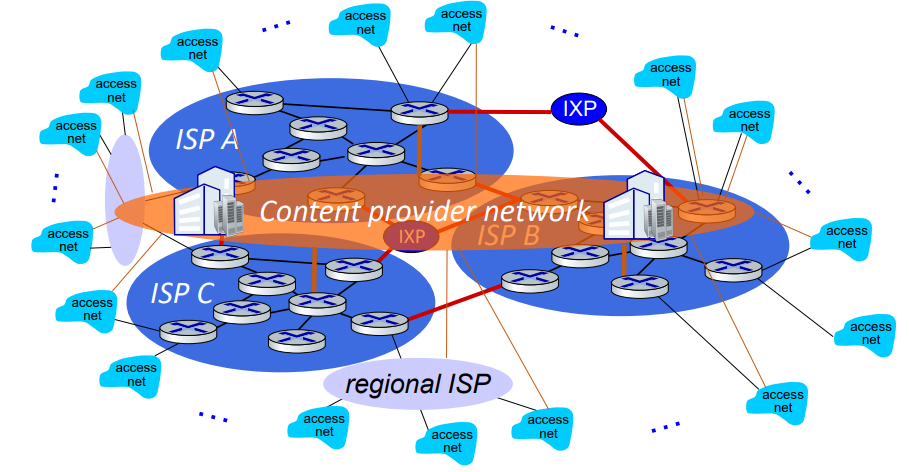
\includegraphics[width =0.85\linewidth]{Images/16.PNG}
\end{center}
Nulla però vieta alle reti dei content provider di accedere anche alle reti degli ISPs globali.
Diamo una versione più generale della gerarchia:
\begin{center}
    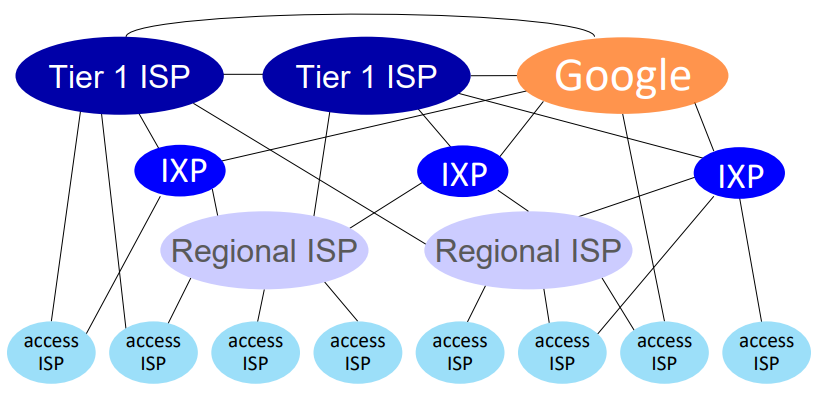
\includegraphics[width =0.85\linewidth]{Images/17.PNG}
\end{center}
Tuttavia, le connessioni possibili \textbf{possono anche non limitarsi a quelle mostrare in figura}.
\subsection{Metriche di performance nelle reti}
Il ritardo e la perdita sono due delle metriche fondamentali per capire la prestazione della rete.
Abbiamo già parlato di \textbf{ritardo di accodamento} e di \textbf{ritardo di trasmissione}, tuttavia essi sono
solo due dei tipi di ritardo che si possono verificare.
\begin{center}
    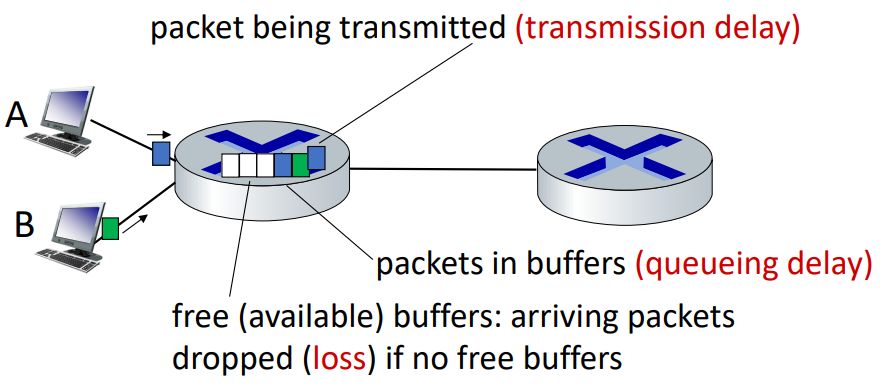
\includegraphics[width =0.70\linewidth]{Images/18.PNG}
\end{center}
Tuttavia ce ne sono delle altre, vediamole tutte: 
\begin{itemize}
    \item \textbf{Ritardo di elaborazione} ($d_{proc}$): quando un pacchetto arriva ad un nodo, devono essere effettuate delle operazioni fondamentali, per esempio \textbf{l'analisi della tabella di inoltro per capire su quale collegamento trasmettere il pacchetto} (lookup).
    Altra operazione è il \textbf{controllo dei bit di errore}: a volte, per colpa di distorsioni o "rumore" sul canale, certi bit di un pacchetto possono essere cambiati (da 0 a 1 e viceversa); il pacchetto quindi risulta malformato. Esistono meccanismi che permettono
    di \textbf{individuare se c'è stato un errore} (e anche di ricostruire il pacchetto originale). Questi metodi sono detti di \textbf{controllo e correzione dell'errore} e richiedono del tempo per essere eseguiti, tendenzialmente nell'ordine dei \textbf{microsecondi} ($10^-6 s$).
    \item \textbf{Ritardo di accodamento} ($d_{queue}$): è il tempo che il pacchetto attende per essere trasmesso. Dipende dal livello di congestione della rete. È tipicamente nell'ordine dei millisecondi
    \item \textbf{Ritardo di trasmissione} ($d_{trans}$): Se abbiamo un pacchetto di lunghezza $L$ che vogliamo trasferire su un collegamento con tasso di trasmissione $R$, allora il ritardo di trasmissione è dato da:
    $$d_{trans} = \frac{L}{R}$$
    \item \textbf{Ritardo di propagazione} ($d_{prop}$): Il ritardo di propagazione è il tempo che necessita un pacchetto per \textbf{propagarsi da un capo all'altro del collegamento}. Questo ritardo dipende dalla lunghezza del collegamento fisico $d$ (espressa in \textbf{metri} (m))
    e dalla \textbf{velocità di propagazione} $s$, che è nell'ordine di grandezza della \textbf{velocità della luce}: $\sim 2 \cdot 10^8 \; m/sec$, e si calcola nel seguente modo:
    $$d_{prop} = \frac{d}{s}$$
\end{itemize}
\begin{center}
    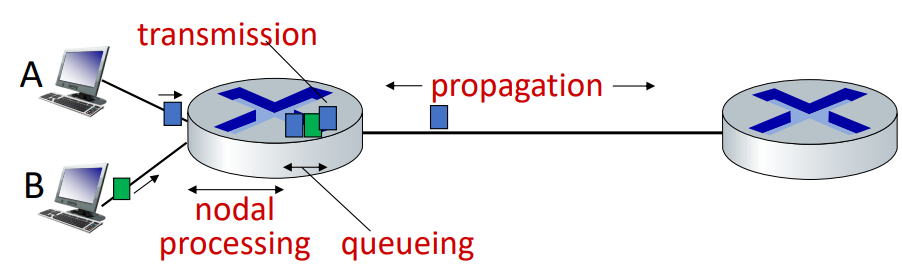
\includegraphics[width =0.70\linewidth]{Images/19.PNG}
\end{center}
Il \textbf{ritardo totale del nodo} (ritardo \textbf{end-to-end}) $d_{nodal}$ è calcolato come la somma di tutti ritardi visti sopra:
$$d_{nodal} = d_{proc} + d_{queue} + d_{trans} + d_{prop}$$
esso è uno delle \textbf{metriche più importanti} e mi permette di valutare le prestazioni della rete. Per calcolare il ritardo ent-to-end bisognerebbe anche tener conto dei \textbf{ritardi introdotti dai sistemi periferici},
che tuttavia non considereremo per questi appunti.
\subsubsection{Ritardo di accodamento e intensità di traffico}
Il ritardo di accodamento ha una caratteristica particolare: mentre tutti gli altri ritardi sono \textbf{analoghi} se considero lo stesso pacchetto trasmesso in due momenti diversi, \textbf{per il ritardo di accodamento non è così}.
Il ritardo di accodamento dipende dallo stato della rete durante la trasmissione. Questo ritardo di solito viene studiato tramite \textbf{metodi statistici}: in particolare, il ritardo di accodamento dipende da un valore che viene chiamato \textbf{intensità di traffico} ("traffic intensity"):
$$\frac{L \cdot \overline{a}}{R} = \frac{\textrm{tasso di arrivo dei pacchetti (bit/s)}}{\textrm{tasso di uscita dei pacchetti (bit/s)}}$$
Dove:
\begin{itemize}
    \item $\overline{a}$ è il \textbf{tasso di arrivo medio dei pacchetti} (pacchetti/s)
    \item $L$ è la \textbf{lunghezza} dei pacchetti (bit/packet)
    \item $R$ è la \textbf{larghezza di banda} del collegamento (bit/s)
\end{itemize}
L'intensità di traffico è \textbf{adimensionale} ed è una quantità non negativa:
\begin{itemize}
    \item Se l'intensità di traffico è \textbf{vicina a 0}, allora il ritardo di accodamento medio sarà piccolo
    \item Se l'intensità di traffico è \textbf{vicina a 1}, allora il ritardo di accodamento medio è grande
    \item Se l'intensità di traffico è \textbf{maggiore di 1}, allora il tasso di arrivo dei pacchetti \textbf{è troppo alto rispetto alla capacità della rete di smaltirli}, quindi il tempo di accodamento medio è \textbf{potenzialmente infinito}
\end{itemize}
\begin{center}
    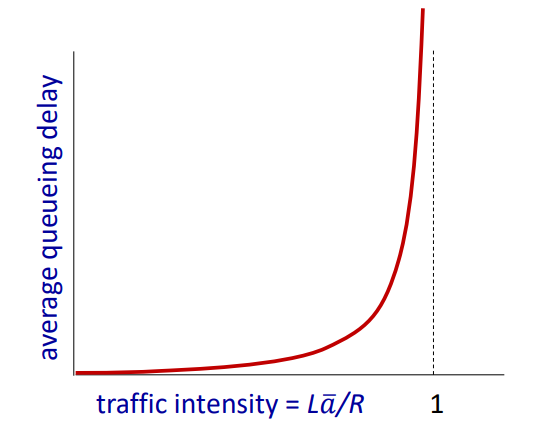
\includegraphics[width =0.50\linewidth]{Images/20.PNG}
\end{center}
\subsubsection{Perdita di pacchetti}
Un'altra metrica di performance fondamentale è la \textbf{perdita di pacchetti}; infatti, idealmente essa dovrebbe essere \textbf{nulla}.
La perdita di pacchetti si verifica quando si ha un buffer overflow sul buffer di accodamento di un nodo.
La perdita di pacchetti può essere mitigata tramite \textbf{meccanismi di ritrasmissione dei pacchetti} da parte del nodo sorgente (tuttavia non è obbligatorio che avvenga).
\begin{center}
    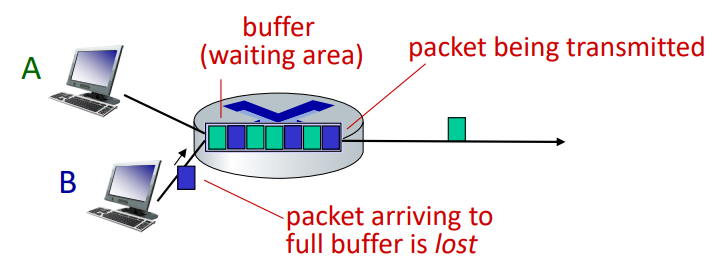
\includegraphics[width =0.70\linewidth]{Images/21.PNG}
\end{center}
Oltre alla perdita per accodamento, \textbf{i pacchetti possono essere scartati dai commutatori} se ci sono stati troppi errori durante la trasmissione oppure se non è previsto un meccanismo di correzione degli errori.
\subsubsection{Throughput}
Il \textbf{throughput} è il \textbf{tasso a cui i bits vengono inviati dal mittente al destinatario}; si calcola in bit/s e viene a volte chiamato \textbf{throughput end-to-end}.
Come si fa a calcolare il throughput?
\begin{itemize}
    \item \textbf{Throughput istantaneo}: tasso di invio \textbf{ad un certo punto nel tempo}
    \item \textbf{Throughput medio}: tasso di invio medio \textbf{su un lungo periodo di tempo}; si può ottenere facendo la media di tutti i valori istantanei o nel seguente modo: supponiamo di voler trasferire un file $F$ dal punto A al punto B; allora il throughput sarà la dimensione del file diviso il tempo che ha impiegato il file ad essere trasferito 
\end{itemize}
Il throughput è una metrica di prestazione "quanto bene" la rete sta andando nella comunicazione tra un mittente ed un destinatario.
\begin{center}
    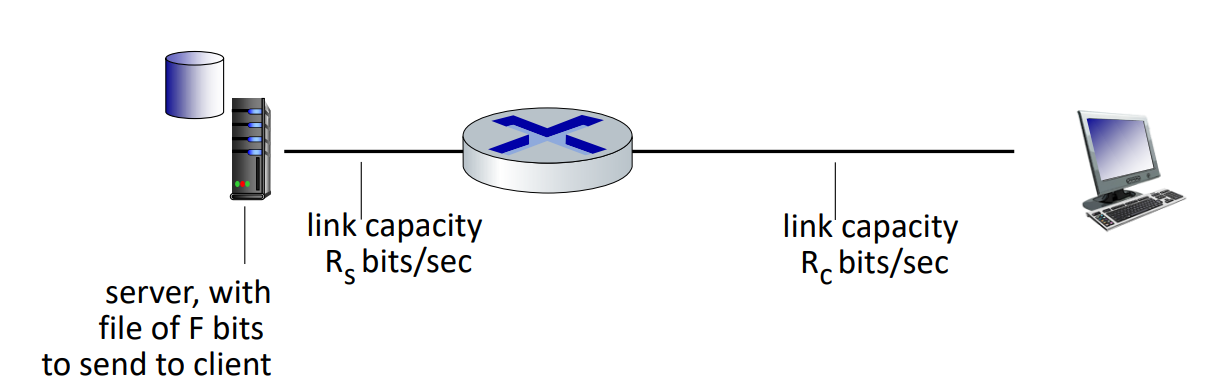
\includegraphics[width =1\linewidth]{Images/22.PNG}
\end{center}
Si possono verificare vari casi:
\begin{itemize}
    \item Se $R_s < R_c$ allora il throughput medio sarà $R_s$. In questo caso, \textbf{non si causerà mai accodamento nel commutatore}
    \item Se $R_s > R_c$ allora il throughput medio sarà $R_c$. In questo caso, potrebbe essere possibile che i \textbf{pacchetti si accodano nel commutatore}
\end{itemize}
In ogni caso, il throughput è vincolato dal collegamento con capacità minore, il quale prende il nome di \textbf{bottleneck link}. Vediamo questo ulteriore scenario:
supponiamo di avere 10 client e 10 server e che essi, per comunicare, passino attraverso un collegamento all'interno della network core con larghezza di banda $R$:
\begin{center}
    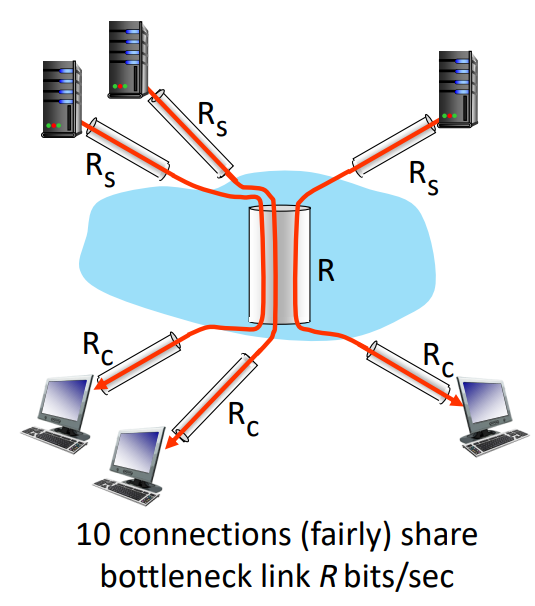
\includegraphics[width =0.40\linewidth]{Images/23.PNG}
\end{center}
In questo caso, il throughput end-to-end per connessione risulta il minimo tra $R_c, R_s,$ e $R/10$, cioè $min\{R_C, R_s, R/10\}$.
Nella pratica, tuttavia, la rete di core ha larghezze di banda \textbf{molto maggiori rispetto ai collegamenti degli hosts}, quindi $R/10$, il più delle volte, sarà comunque molto maggiore di $R_s$ e $R_c$.
Ciò significa che, molto spesso, il bottleneck è dato dai collegamenti di accesso.
\subsection{Strato protocollare e modelli di servizio}
Le reti sono dei sistemi molto complessi con diverse componenti che interagiscono fra loro
\begin{itemize}
    \item Hosts
    \item Routers
    \item Collegamenti di diverso tipo e scopo
    \item Applicazioni
    \item Protocolli
    \item Hardware e Software
\end{itemize}
C'è allora un modo intelligente per \textbf{strutturare e discutere le reti}?
Un modo è una \textbf{struttura a strati}, in cui ogni servizio viene implementato tramite \textbf{azioni interne allo strato} e ogni servizio fa affidamento ai servizi \textbf{appartenenti al livello sottostante per implementare le proprie operazioni e garantirne il funzionamento}.
Inoltre, i vari strati sono \textbf{indipendenti l'uno dall'altro}, nel senso che, in caso di modifiche a come vengono implementati i servizi in uno strato, gli altri strati \textbf{non vengono influenzati dalla modifica}.
L'approccio a strati quindi permette di approcciarsi alla modellazione e alla discussione di sistemi complessi:
\begin{itemize}
    \item La sua \textbf{struttura esplicita} permette l'identificazione e le \textbf{relazioni fra le varia componenti del sistema}. Crea inoltre un \textbf{modello di riferimento a strati} per la discussione
    \item Permette la \textbf{modularizzazione} del sistema e quindi rende più semplice l'aggiornamento e la manutenzione di questo
    \begin{itemize}
        \item I cambiamenti nell'implementazione dei servizi di uno strato sono \textbf{trasparenti al resto del sistema} e quindi non lo influenzano
    \end{itemize}
\end{itemize}
Ciò che è stato definito per internet prende il nome di \textbf{pila (o stack) protocollare di internet} e prevede l'esistenza di 5 diversi strati, numerati dal basso verso l'alto:
\begin{center}
    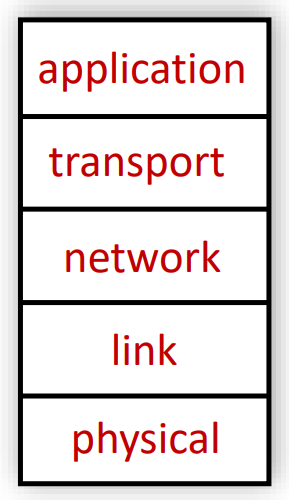
\includegraphics[width =0.15\linewidth]{Images/24.PNG}
\end{center}
Vediamoli nel dettaglio:
\begin{itemize}
    \item \textbf{LIVELLO 5: APPLICATIVO}: Tutti i protocolli volti al supporto alle applicazioni di rete (HTTP, SMTP, DNS ecc..)
    \item \textbf{LIVELLO 4: TRASPORTO}: Ha il compito di effettuare un trasferimento di dati tra macchine che si trovano su reti differenti. Esempio di protocolli a questo livello sono TCP e UDP
    \item \textbf{LIVELLO 3: RETE}: Offre il servizio fondamentale di \textbf{instradamento} tra sorgente e destinazione. Protocollo fondamentale a questo livello è \textbf{Internet Protocol} (IP)
    \item \textbf{LIVELLO 2: COLLEGAMENTO}: Ha il compito di trasferire i dati tra \textbf{due entità di rete adiacenti}, cioè su un collegamento. Protocolli a questo livello sono, per esempio, Ethernet e 802.11(WiFi).
    \item \textbf{LIVELLO 1: FISICO}: Trasporto fisico dei bit su un cavo (o canale radio)
\end{itemize}
\subsubsection{Servizi, Stratificazione e Incapsulamento}
Come si può andare ad implementare i vari protocolli che garantiscono il funzionamento dei servizi ad ogni livello?
Un concetto fondamentale da introdurre a questo scopo è quello dell'\textbf{incapsulamento}: le applicazioni si devono
scambiare messaggi per realizzare i propri servizi, e per farlo devono basarsi sui servizi offerti dal \textbf{livello di trasporto}
\begin{center}
    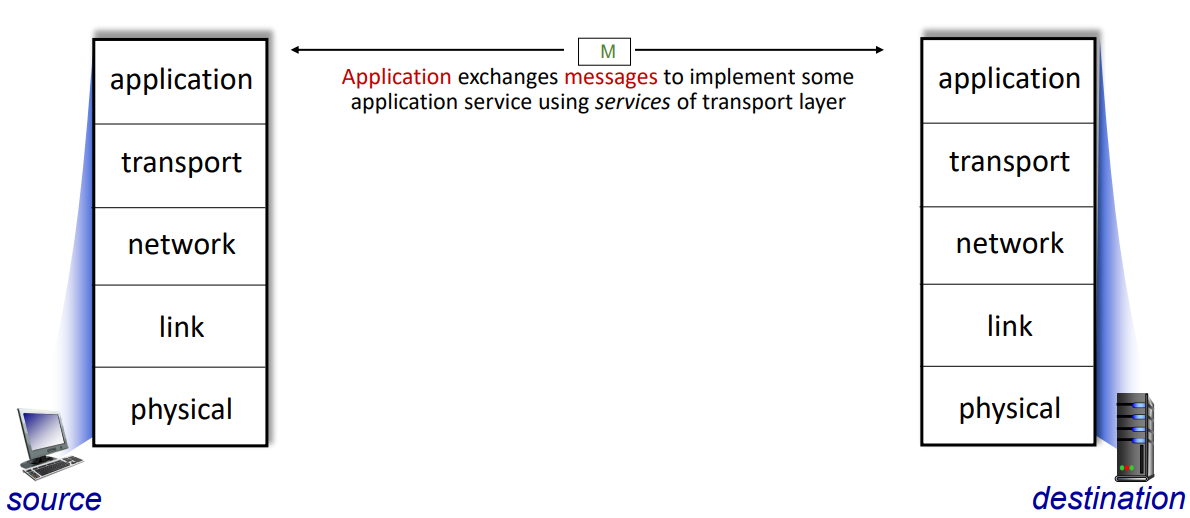
\includegraphics[width =1\linewidth]{Images/25.PNG}
\end{center}
Il messaggio viene quindi passato al livello di trasporto, il quale \textbf{aggiunge un'intestazione (operazione di incapsulamento)} che va ad implementare il servizio a livello di trasporto:
\begin{center}
    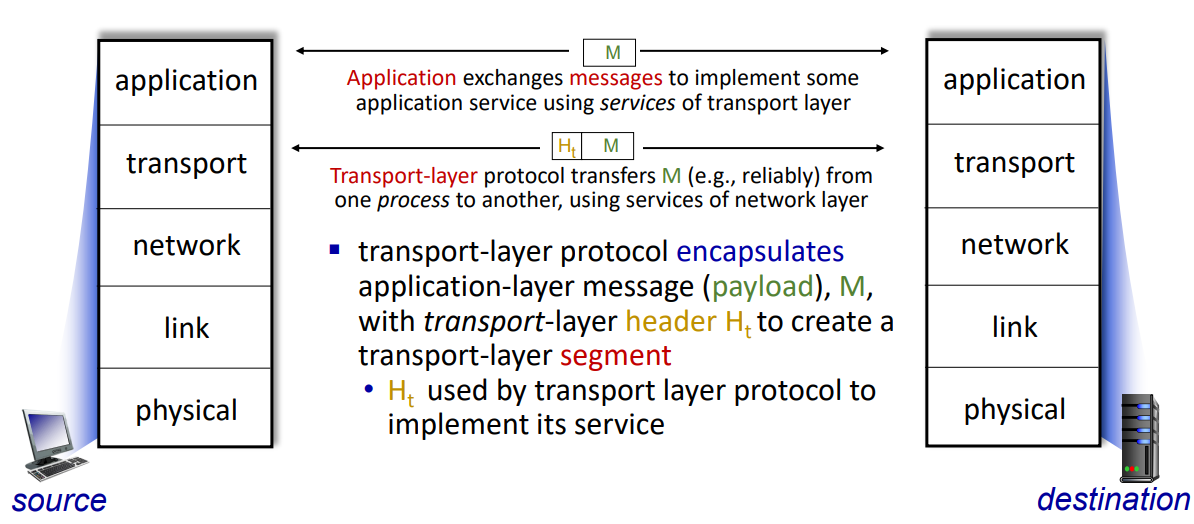
\includegraphics[width =1\linewidth]{Images/26.PNG}
\end{center}
A sua volta, il livello di trasporto usa \textbf{i servizi del livello di rete}, quindi passerò il nuovo \textbf{segmento} al livello di rete, il quale aggiungerà un'ulteriore intestazione:
\begin{center}
    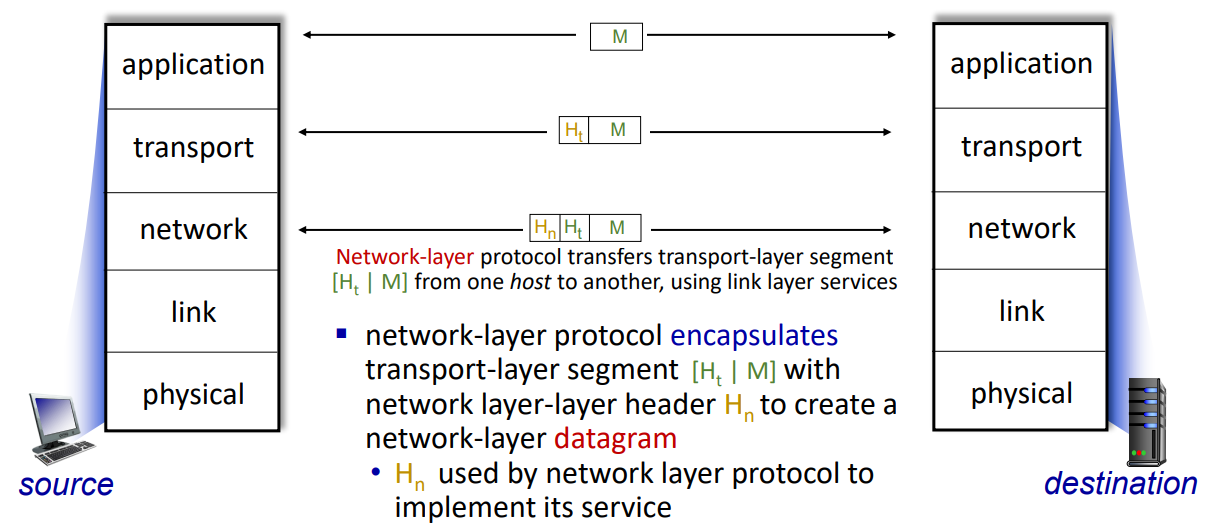
\includegraphics[width =1\linewidth]{Images/27.PNG}
\end{center}
Da notare che a questo livello \textbf{il payload contiene anche l'header del trasporto}, e sarà così anche per le prossime operazioni.
Lo strato di rete si basa sui \textbf{servizi offerti dal livello di collegamento} per implementare i propri, quindi passa il nuovo \textbf{datagramma} ottenuto al livello di collegamento:
\begin{center}
    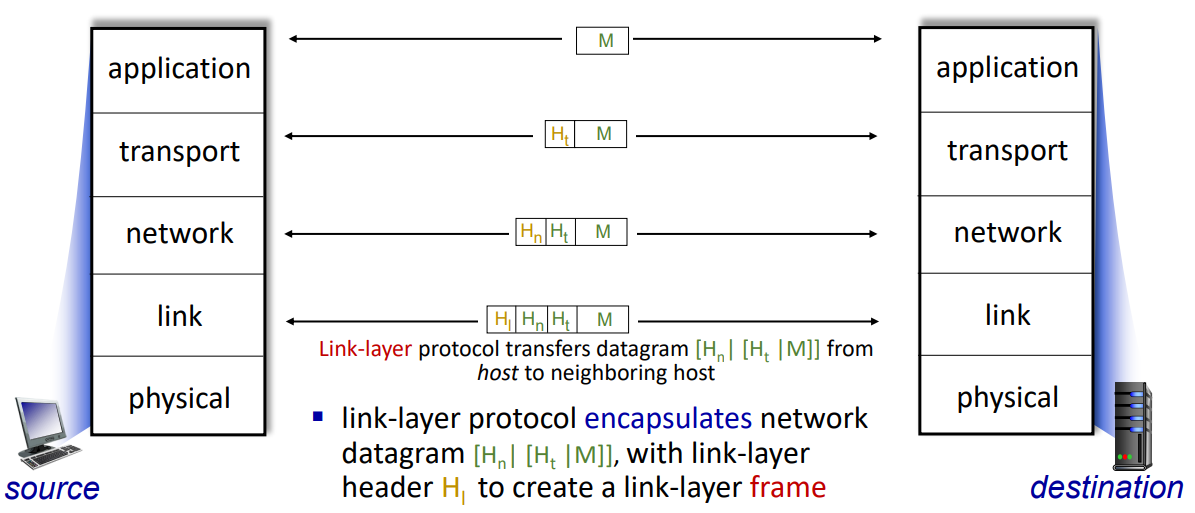
\includegraphics[width =1\linewidth]{Images/28.PNG}
\end{center}
Infine, il pacchetto verrà passato al livello fisico e quindi trasmesso al destinatario.
Come abbiamo già accennato, i pacchetti hanno  nome diverso in strati diversi:
\begin{center}
    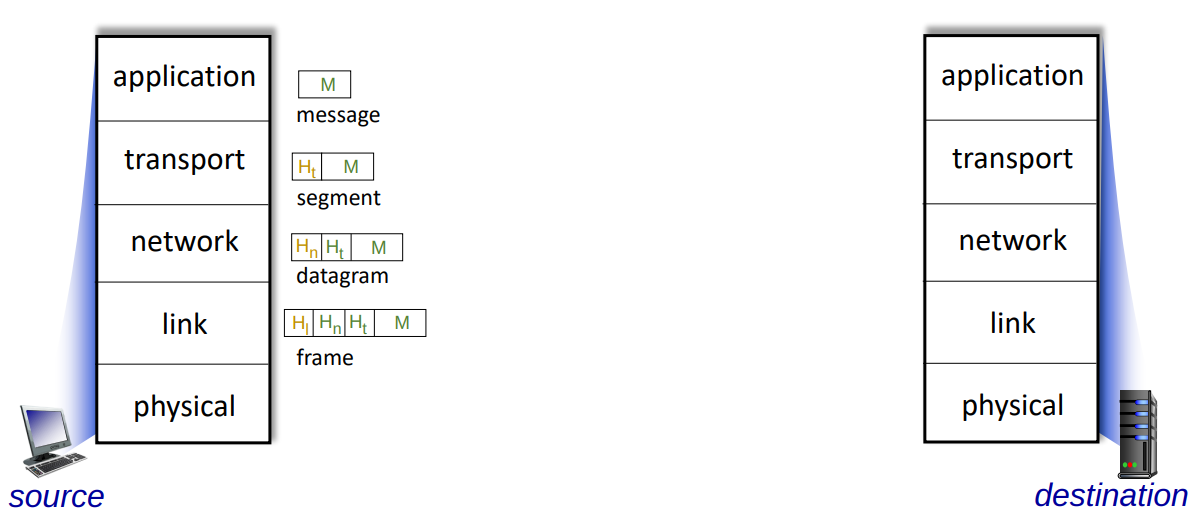
\includegraphics[width =1\linewidth]{Images/29.png}
\end{center}
Man mano che si scende nella pila protocollare, vengono aggiunti nuovi bit di intestazione, i quali servono per \textbf{far funzionare i servizi di rete}.
L'insieme di tutti i bit aggiunti da ogni strato prende il nome di \textbf{overhead} del pacchetto. Poiché il throughput viene misurato \textbf{a livello applicativo},
non si avrà mai, a livello pratico, \textbf{una misura di throughput massima} poiché non vengono contati i bit di overhead. Dopo l'operazione di \textbf{incapsulamento} del messaggio
e di trasmissione su cavo fisico, avviene sul sistema ricevente un'operazione di \textbf{decapsulamento} del messaggio:
\begin{center}
    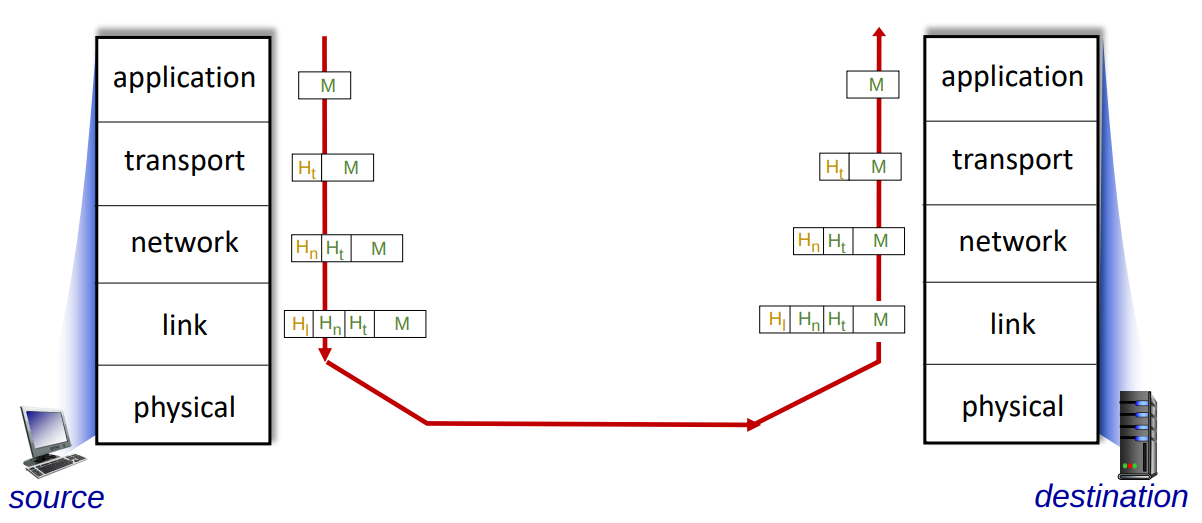
\includegraphics[width =1\linewidth]{Images/30.png}
\end{center}
I sistemi periferici sono sempre in grado di interpretare tutti gli strati della pila protocollare; questo però non è vero per i \textbf{commutatori}, che "parlano" fino al \textbf{livello 2} se sono
degli \textbf{switch} e fino al \textbf{livello 3} se sono dei \textbf{router}:
\begin{center}
    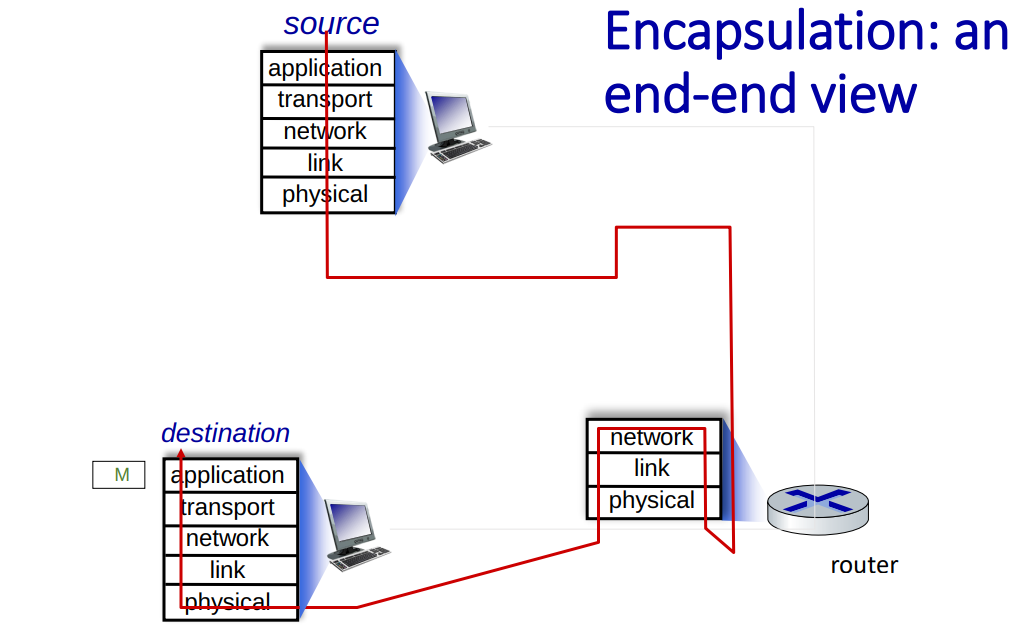
\includegraphics[width = 0.80\linewidth]{Images/31.png}
\end{center}
\section{Strato applicativo: Domain Name System}
Lo strato applicativo ha la funzione di interfacciare e fornire servizi di connettività per i \textbf{processi delle applicazioni}. Il numero
di protocolli presenti in questo strato è altissimo; in questi appunti, tuttavia, ci concentreremo sul protocollo \textbf{DNS}, il quale è una funzionalità chiave di internet, in particolare
se si pensa ad esso come \textbf{fornitore di servizi web}. Quando inseriamo il \textbf{nome} di un sito nel browser, ciò che è avviene è lo scatenamento di un meccanismo che permette al computer
di ottenere \textbf{l'indirizzo IP} (quindi l'indirizzo a livello di rete) associato al server che deve fornire la pagina web richiesta. Per ottenere questo indirizzo IP, non si può pensare di conoscere
ogni indirizzo esistente, quindi è necessario un meccanismo che ci permette di reperirlo: il \textbf{Domain Name System} (DNS). Il DNS permette di effettuare la traduzione dall'\textbf{host name} (i nomi "human readable" dei siti)
all'indirizzo IP del server associato che dovrà fornire al richiedente il contenuto. Come funziona quindi la traduzione? Essa sfrutta la \textbf{gerarchia} di un numero molto elevato di \textbf{server DNS} (che prendono anche il nome di \textbf{name servers}),
i quali andranno a \textbf{risolvere} (tradurre) gli host name in indirizzi IP. Poiché il DNS è un protocollo a livello applicativo, la complessità di questa operazione si trova \textbf{interamente ai confini della rete}.
Il DNS funziona nel seguente modo:
\begin{center}
    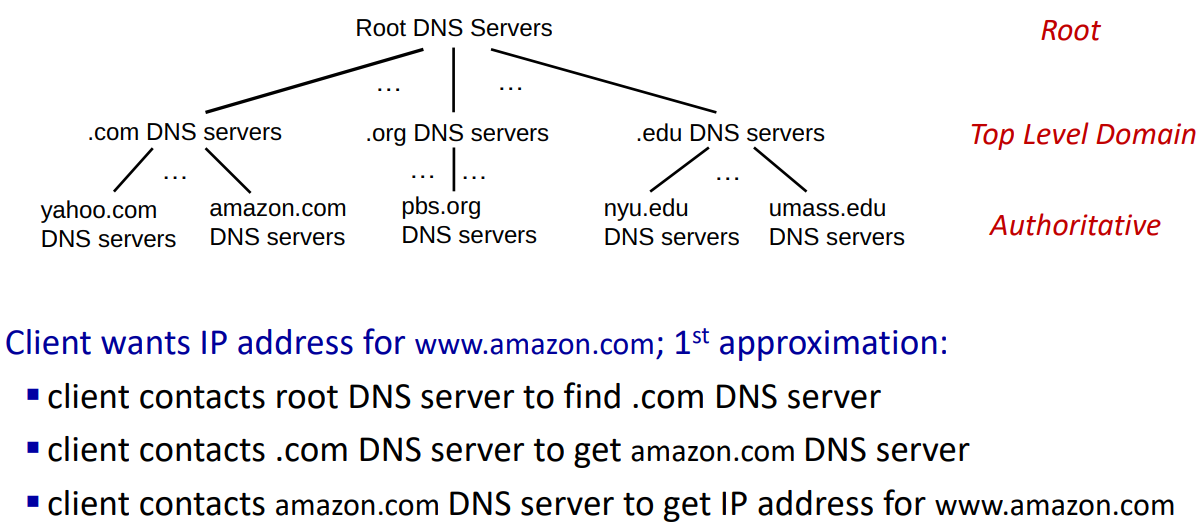
\includegraphics[width = 0.90\linewidth]{Images/32.png}
\end{center}
abbiamo quindi un sistema distribuito che si articola su \textbf{3 livelli}:
\begin{itemize}
    \item \textbf{Root DNS servers}: sono la radice dell'albero gerarchico
    \item \textbf{Top Level Domain (TLD) DNS Servers}: sono responsabili della risoluzione dei \textbf{Top Level Domains}(TLDs); come per esempio .com, .net, .it, ...
    \item \textbf{Authoritative DNS Servers}: Responsabili di risolvere gli indirizzi per i vari domini autoritativi (es. amazon.com, google.com ecc...)
\end{itemize}
Questi 3 livelli collaborano tra loro per risolvere il nome richiesto.
\subsection{Root DNS Servers}
I root DNS server stanno alla radice del sistema DNS e senza la loro esistenza \textbf{è fondamentale per l'esistenza del web}.
In tutto, esistono 13 root name servers "logici", gestiti da \textbf{12 provider differenti}; a loro volta ognuno di questi root dns server è replicato
più volte nel globo. È fondamentale avere repliche dei root name server geograficamente sparse che possono essere acceduti dai vari luogo del mondo.
\begin{center}
    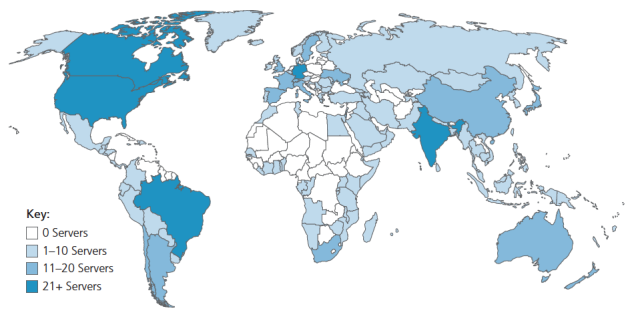
\includegraphics[width = 0.70\linewidth]{Images/33.png}
\end{center}
\subsection{Top Level DNS servers e Authoritative DNS servers}
Ogni TLD DNS server è responsabile per la risoluzione dei TLD, inclusi quelli nazionali (.it, .de. .pl, ...).
I DNS server autoritativi invece è importate specificare che \textbf{possono essere mantenuti dall'organizzazione che detiene il dominio}
oppure \textbf{possono essere mantenuti da un service provider}. Il loro compito è di risolvere le richieste relative a tutte le pagine appartenenti
al loro dominio.
\subsection{Local DNS name servers}
Quando vi è la necessità di contattare il DNS per risolvere un dominio,la prima cosa che viene fatta è contattare il \textbf{DNS server locale}, a cui viene
demandata di fatto questa risoluzione. Il DNS server locale ha un ruolo fondamentale: esistono DNS server locali forniti da ISP, che di solito sono l'opzione di default,
tuttavia un utente può benissimo cambiare il proprio DNS server locale ad uno fornito da un'organizzazione terza. Il DNS server locale tendenzialmente fornisce due servizi:
\begin{itemize}
    \item Mantiene una cache delle associazioni nome-indirizzo IP. Questa cache viene costruita a partire dalle varie richieste dei sistemi terminali e di solito le associazioni
    vengono mantenute per 2 giorni. Il DNS server locale quindi risponderà direttamente alle richieste del client, senza quindi interpellare la gerarchia del DNS, se il nome richiesto è presente
    nella sua cache.
    \item In caso il nome richiesto non sia presente in cache, il DNS server locale procederà ad inoltrare la richiesta alla gerarchia del DNS; una volta ottenuta risposta, procederà a comunicarla al client
\end{itemize}
Ogni richiesta al DNS prende il nome di \textbf{query}.
\subsection{DNS name resolution: Iterated query}
Ci sono due modi per effettuare query al DNS.
Il modo che prende il nome di \textbf{query iterativa} è quello che viene usato più spesso.
In questo metodo, il local DNS server ha \textbf{il maggior carico} dal punto di vista delle richieste da servire.
\begin{center}
    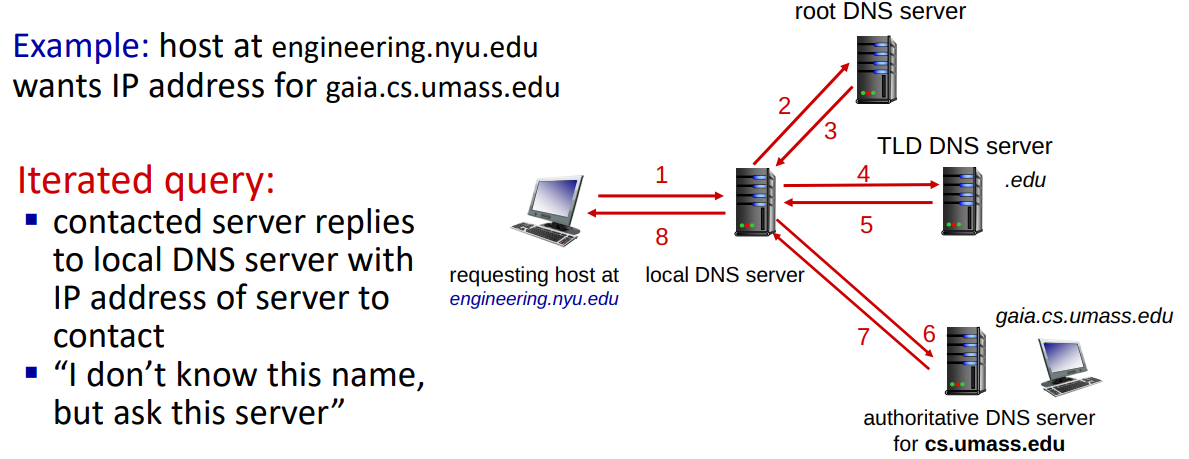
\includegraphics[width = 1\linewidth]{Images/34.png}
\end{center}
\newpage \noindent
Analizziamo nel dettaglio ogni passaggio:
\begin{enumerate}
    \item L'host chiede al DNS server locale di risolvere un certo nome in un indirizzo IP
    \item Il DNS server locale chiede al DNS server root di risolvere il nome
    \item Il DNS server root indica al server DNS server locale quale TLD DNS server può risolvere la sua richiesta
    \item Il DNS server locale chiede al TLD DNS server indicato di risolvere il nome
    \item Il TLD DNS server indica al server DNS locale quale DNS server autoritativo può risolvere la sua richiesta
    \item Il DNS server locale chiede al server DNS autoritativo di risolvere il nome
    \item Il DNS server autoritativo restituisce l'indirizzo IP associato al nome indicato
    \item Il DNS server locale restituisce l'indirizzo IP al client
\end{enumerate}
Ogni passaggio di questo processo è inoltre \textbf{trasparente all'utente}.
\subsection{DNS name resolution: recursive query}
In una query ricorsiva, la risoluzione viene effettuata, in modo gerarchico, dal DNS server di livello superiore.
Il peso delle richieste quindi grava sulla \textbf{struttura gerarchica del DNS}.
\begin{center}
    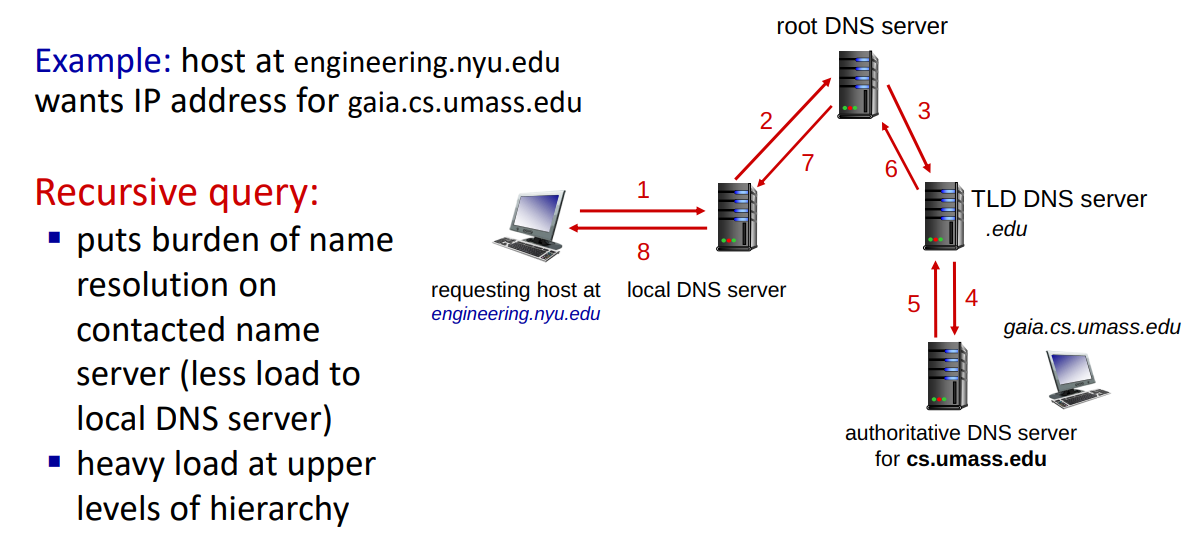
\includegraphics[width = 1\linewidth]{Images/35.png}
\end{center}
Vediamo ogni passo in dettaglio:
\begin{enumerate}
    \item Il client chiede al DNS server locale di risolvere il nome
    \item Il DNS server locale chiede al DNS server di root di risolvere il nome
    \item Il DNS server di root chiede al TLD DNS Server corrispondente di risolvere il nome
    \item Il TLD DNS server chiede al DNS server autoritativo corrispondente di risolvere il nome
    \item Il DNS server autoritativo restituisce l'IP richiesto al TLD DNS server
    \item Il TLD DNS server restituisce la risposta ottenuta al root DNS server
    \item Il root DNS server restituisce la risposta ottenuta al DNS server locale
    \item Il DNS server locale restituisce la risposta ottenuta al client
\end{enumerate}
Solitamente, questo meccanismo non si utilizza poiché tendenzialmente i TLD DNS server, per loro natura, si trovano a gestire
un alta quantità di traffico, quindi un meccanismo di risposta ricorsivo porrebbe ulteriore peso su di essi. Si tende quindi
a cercare di mantenere il peso sui DNS server locali, i quali tendenzialmente gestiscono una quantità di traffico molto minore.
\section{Livello di trasporto}
I servizi del livello di trasporto offrono:
\begin{itemize}
    \item \textbf{comunicazione logica} tra processi su host diversi, cioè processi su macchine diversi possono comunicare come se fossero direttamente connessi fra loro
    \item Le azioni effettuate dai protocolli di trasporto nei sistemi periferici sono:
    \begin{itemize}
        \item \textbf{Mittente}: il livello di trasporto deve prendere i messaggi applicativi, eventualmente \textbf{dividerli in parti più piccole}, incapsularli in quelli che prendono il nome di \textbf{segmenti}
        \item \textbf{Destinatario}: il livello di trasporto \textbf{riassembla i segmenti} per ricostruire il messaggio originale e poi passa il messaggio ricostruito al livello applicativo
    \end{itemize}
\end{itemize}
Come si differenzia il servizio di comunicazione tra processi offerto dal livello di trasporto dal servizio offerto dal livello di rete?
\begin{itemize}
    \item A \textbf{livello di rete}, abbiamo una comunicazione logica tra \textbf{hosts}
    \item A \textbf{livello di trasporto}, estende la comunicazione logica offerta dal livello di rete, migliorandola a una comunicazione tra \textbf{processi su host differenti}  
\end{itemize}
\subsection{Sockets}
Una \textbf{socket} è un "varco" che permette ai processi a livello applicativo di comunicare con il livello di trasporto e di inviare i messaggi verso destinatari
usando lo stack protocollare di internet. Quando quindi un processo deve mandare un messaggio in rete, \textbf{lo fa passare attraverso una socket}; vengono poi sfruttati i servizi
offerti dal livello di trasporto per fare in modo che il messaggio sia recapitato \textbf{ad un'altra socket dal lato del destinatario} (ci sono quindi almeno sempre due socket in una comunicazione tra processi).
Dal punto di vista formale, una socket è \textbf{un'interfaccia} che permette di interfacciare il livello applicativo con il livello di trasporto. La cosa particolare della socket è che, da un lato la parte della socket
che si \textbf{interfaccia con i processi applicativi} può essere controllata da chi sviluppa l'applicazione (può aprirla, chiuderla, ...), dall'altro la parte che si interfaccia con il livello di trasporto è \textbf{controllata dal sistema operativo},
il quale implementa lo stack protocollare.
\begin{center}
    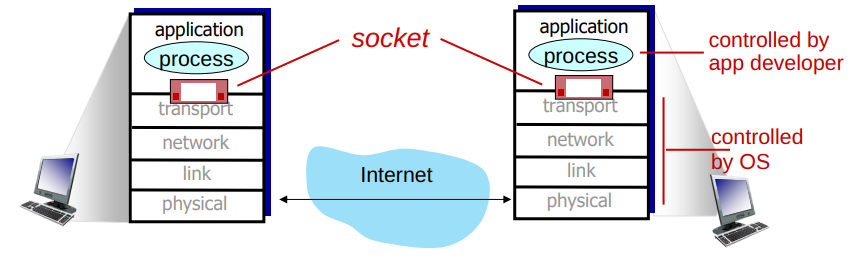
\includegraphics[width = 1\linewidth]{Images/36.png}
\end{center}
\begin{center}
    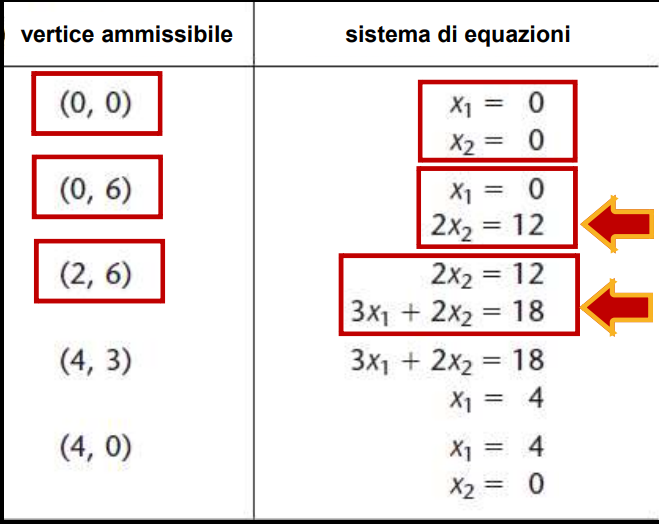
\includegraphics[width = 1\linewidth]{Images/37.png}
\end{center}
\begin{center}
    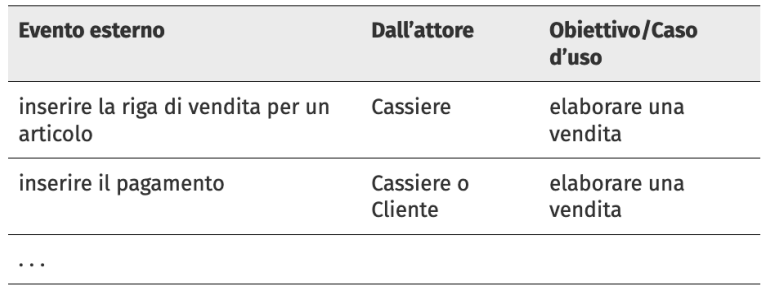
\includegraphics[width = 1\linewidth]{Images/38.png}
\end{center}
\subsection{I principali protocolli di trasporto}
Vi sono due principali protocolli di trasporto:
\begin{itemize}
    \item \textbf{Transmission Control Protocol (TCP)}: Fornisce un servizio di \textbf{consegna dei dati affidabile e in ordine}.
    Offre meccanismi di \textbf{controllo della congestione, controllo di flusso} e di \textbf{inizializzazione della connessione} (TCP è un protocollo \textbf{connection oriented}).
    TCP è adatto alle applicazioni dette \textbf{elastiche}, cioè poco sensibili al ritardo ma \textbf{molto sensibile alla perdita di pacchetti}
    \item \textbf{User Datagram Protocol (UDP)}: Protocollo di trasporto "\textbf{best-effort}" il quale è un'estensione "senza fronzoli" del protocollo IP. 
    Il protocollo è di tipo \textbf{connectionless} ed è adatto alle applicazioni dette \textbf{real-time}: poco sensibili
    alla perdita di pacchetti (in un certo grado) ma \textbf{molto sensibili al ritardo}
\end{itemize}
Nessuno dei due protocolli \textbf{garantisce qualcosa in termini di ritardo}, cioè nessuno dei due garantisce che i pacchetti saranno
consegnati con un ritardo massimo di $n$ secondi. Allo stesso modo, nessuno dei due protocolli garantisce nulla riguardo alla \textbf{banda}: nessuno dei due
garantisce che la comunicazione avvenga a certi bit/s.
\subsection{Multiplexing e Demultiplexing}
Quando si parla di Multiplexing in generale si parla di un'operazione che porta ad unire \textbf{più flussi} in un unico flusso.
Nel caso specifico del livello di trasporto, dobbiamo garantire che il servizio di multiplexing/demultiplexing sia \textbf{garantito} poiché mi permette
di \textbf{estendere logicamente la comunicazione ai processi}. 
\begin{center}
    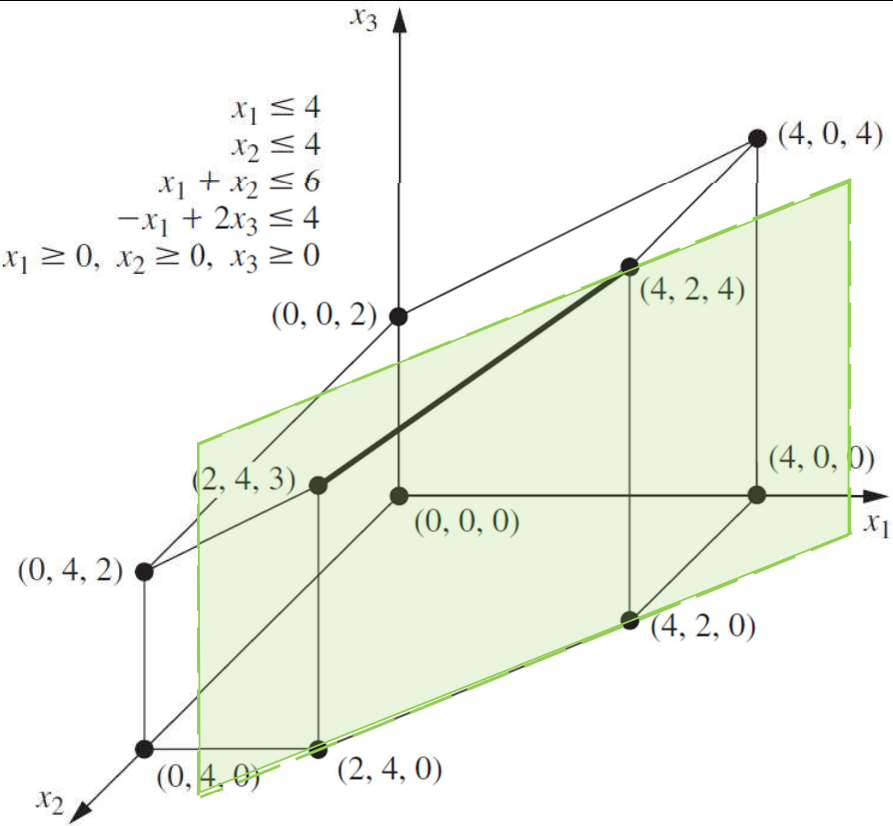
\includegraphics[width = 0.90\linewidth]{Images/39.png}
\end{center}
\begin{center}
    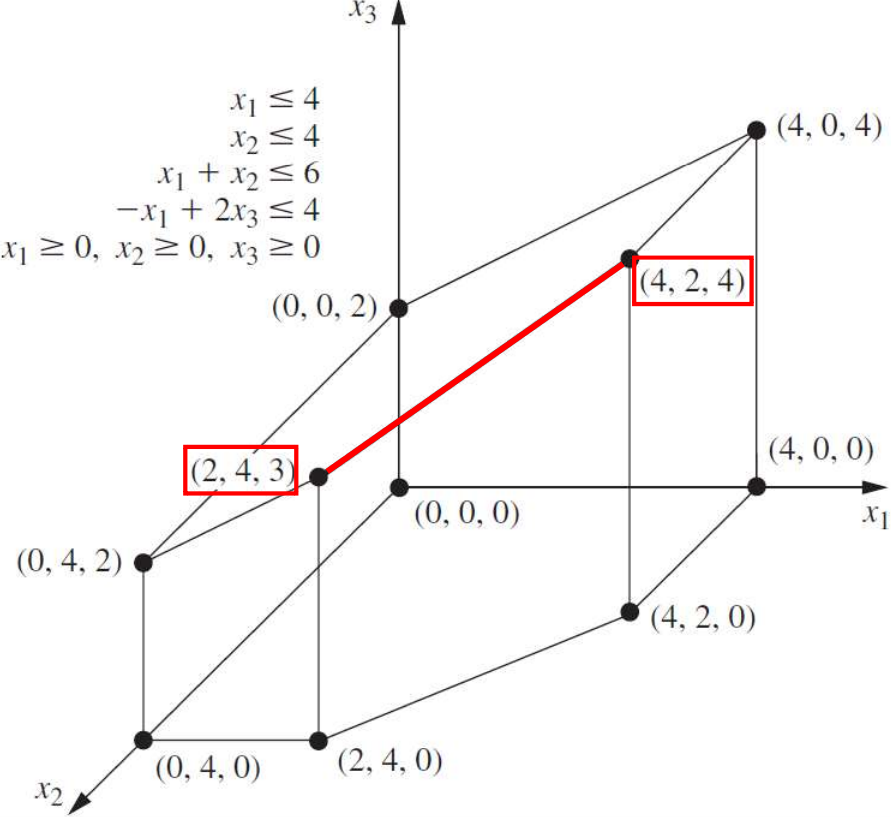
\includegraphics[width = 0.90\linewidth]{Images/40.png}
\end{center}
quindi, l'operazione di multiplazione \textbf{porta ad aggiungere un header ai messaggi provenienti dai processi}, in modo tale che essi siano \textbf{distinguibili} una volta che arrivano al livello di rete; il quale \textbf{non ha conoscenza di quale processo ha generato quale segmento}
ma si preoccupa solamente di consegnare il pacchetto \textbf{all'host corretto}. L'informazione che permette di distinguere i pacchetti è la \textbf{porta di destinazione}. Il livello di trasporto si vedrà recapitati segmenti, dal livello di rete, che avranno
nel loro header dell'informazione relativa alla porta di destinazione; l'operazione di \textbf{demultiplazione} permette, a livello di trasporto, di inoltrare \textbf{verso la socket corretta} segmenti diretti verso \textbf{processi differenti}.
In particolare, l'operazione di \textbf{demultiplazione} funziona nel seguente modo:
\begin{itemize}
    \item L'host riceve i \textbf{datagrammi IP}:
    \begin{itemize}
        \item Ogni datagramma ha un indirizzo IP sorgente e un indirizzo IP destinatario
        \item Ogni datagramma trasporta un \textbf{segmento del livello di trasporto}
        \item Ogni segmento ha una \textbf{numero di porta sorgente e il numero della porta di destinazione}
    \end{itemize}
    \item L'host mittente usa \textbf{l'indirizzo IP e il numero di porta} per inviare i segmenti alla socket appropriata
\end{itemize}
\subsubsection{Connectionless demultiplexing}
Quando si va a creare una socket, \textbf{bisogna specificare attraverso su quale porta essa è raggiungibile}.
La socket di destinazione è \textbf{univocamente identificata} da una coppia di valori:
\begin{enumerate}
    \item \textbf{L'indirizzo IP di destinazione}
    \item \textbf{Il numero della porta di destinazione}
\end{enumerate}
Quando l'host destinatario riceve un segmento UDP:
\begin{itemize}
    \item Controlla il numero della porta di destinazione nel segmento
    \item Invia il segmento UDP alla socket con quella porta
\end{itemize}
I datagrammi IP/UDP con \textbf{la stessa porta di destinazione e stesso indirizzo IP di destinazione}, anche se da indirizzi IP sorgenti differenti e/o con differenti numeri di porta sorgente, saranno
\textbf{inviati alla stessa socket} dell'host destinatario.
\begin{center}
    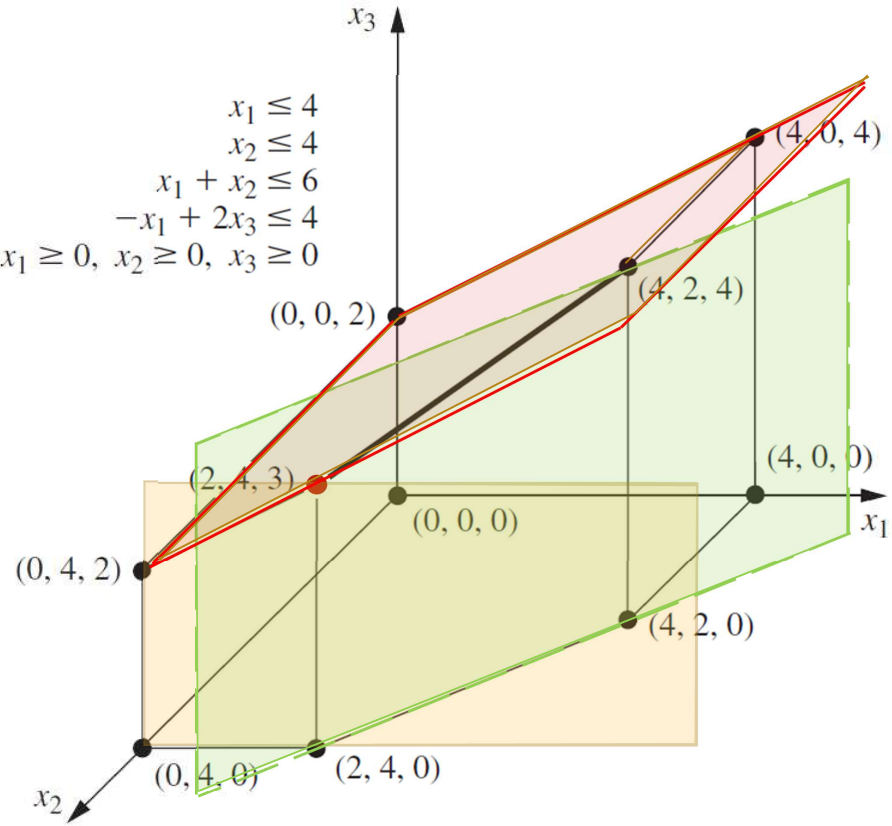
\includegraphics[width = 0.90\linewidth]{Images/41.png}
\end{center}
\subsubsection{Connection-oriented demultiplexing}
A differenza dei protocolli connectionless, una socket è qui identificata \textbf{da una quadrupla}:\
\begin{itemize}
    \item \textbf{Indirizzo IP sorgente}
    \item \textbf{Numero di porta sorgente}
    \item \textbf{Indirizzo IP destinatario}
    \item \textbf{Numero della porta di destinazione}
\end{itemize}
Quando viene effettuata la demultiplazione, allora \textbf{tutti e 4 i valori} verranno usati per inviare il pacchetto alla socket corretta.
Ciò significa che qui si avrà \textbf{una socket dedicata ad ogni connessione}. I server \textbf{possono supportare più socket TCP simultaneamente} e:\
\begin{itemize}
    \item Ogni socket è identificata da una sua quadrupla
    \item Ad ogni socket è \textbf{associato un diverso client comunicante}
\end{itemize}
\begin{center}
    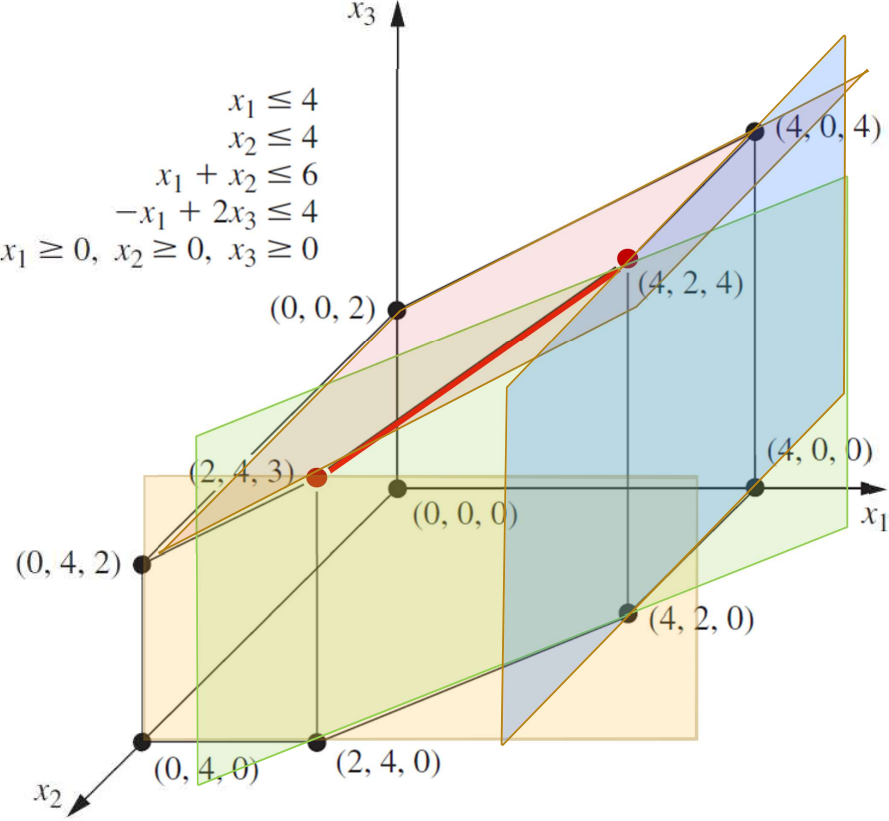
\includegraphics[width = 0.90\linewidth]{Images/42.png}
\end{center}
\subsection{User Datagram Protocol (UDP)}
\textbf{User Datagram Protocol} (UDP) è, di fatto, un'estensione "senza fronzoli" e "minimale" del protocollo IP.
UDP fornisce un servizio di trasporto \textbf{"best effort"}, quindi i segmenti di UDP potrebbero essere:
\begin{itemize}
    \item Persi 
    \item Consegnati in disordine all'applicazione
\end{itemize}
È un \textbf{protocollo connectionless}:
\begin{itemize}
    \item Nessun "handshaking" (inizializzazione della connessione) tra il mittente e il destinatario
    \item Ogni segmento UDP viene gestito indipendentemente dagli altri
\end{itemize}
Perché è necessaria l'esistenza  di UPD?
\begin{itemize}
    \item Nessuna necessità di stabilire una connessione (il che può aggiungere ritardi)
    \item È \textbf{semplice}: nessuno stato di connessione al mittente e al destinatario
    \item \textbf{Dimensioni dell'intestazione piccole}
    \item \textbf{Nessun controllo di congestione}
    \begin{itemize}
        \item UDP può \textbf{trasmettere quanto veloce si vuole}
        \item Può funzionare in casi di congestione della rete (più o meno, comunque fatica in caso di congestione molto elevata)
    \end{itemize}
\end{itemize}
L'header di UDP ha la seguente struttura:
\begin{center}
    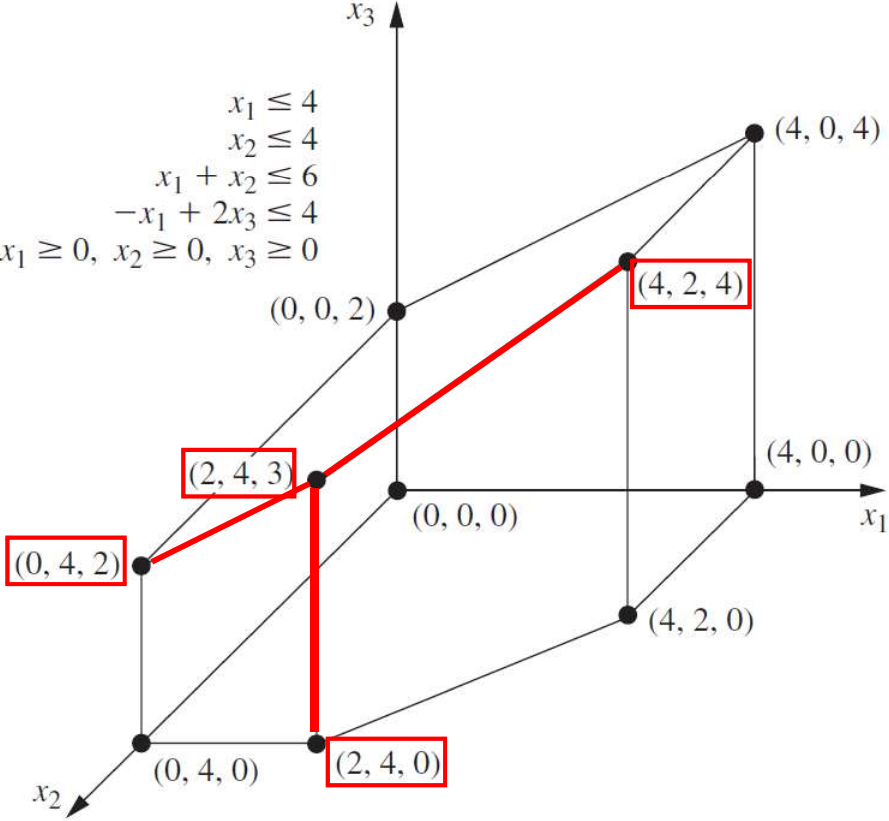
\includegraphics[width = 0.80\linewidth]{Images/43.png}
\end{center}
Facciamo qualche considerazione:
\begin{itemize}
    \item L'header è quindi di \textbf{64 bit}, ed ogni campo è lungo \textbf{16 bit}.
    \item Posso avere $2^{16} - 1$ possibili porti di sorgente e destinazione (la porta con tutti 0 non è tendenzialmente una porta valida)
    \item Includendo l'header, al più posso avere $2^{16} - 1$ byte differenti in un segmento UDP
    \item Il checksum si calcola nel seguente modo: si considerino gruppi di 16 bit del segmento; si sommino modulo 2 e si faccia il complemento di essa.
    Lato destinatario, si effettua la stessa operazione e poi si somma con il checksum: se si ottengono tutti 0 allora non ci sono stati errori.
\end{itemize}
\subsection{Principi del trasferimento dati affidabile}
Per servizio di dati affidabile si intende un servizio di trasporto in cui i dati \textbf{vengono consegnati senza perdite e senza errori}.
Dal punto di vista astratto vogliamo avere la seguente situazione:
\begin{center}
    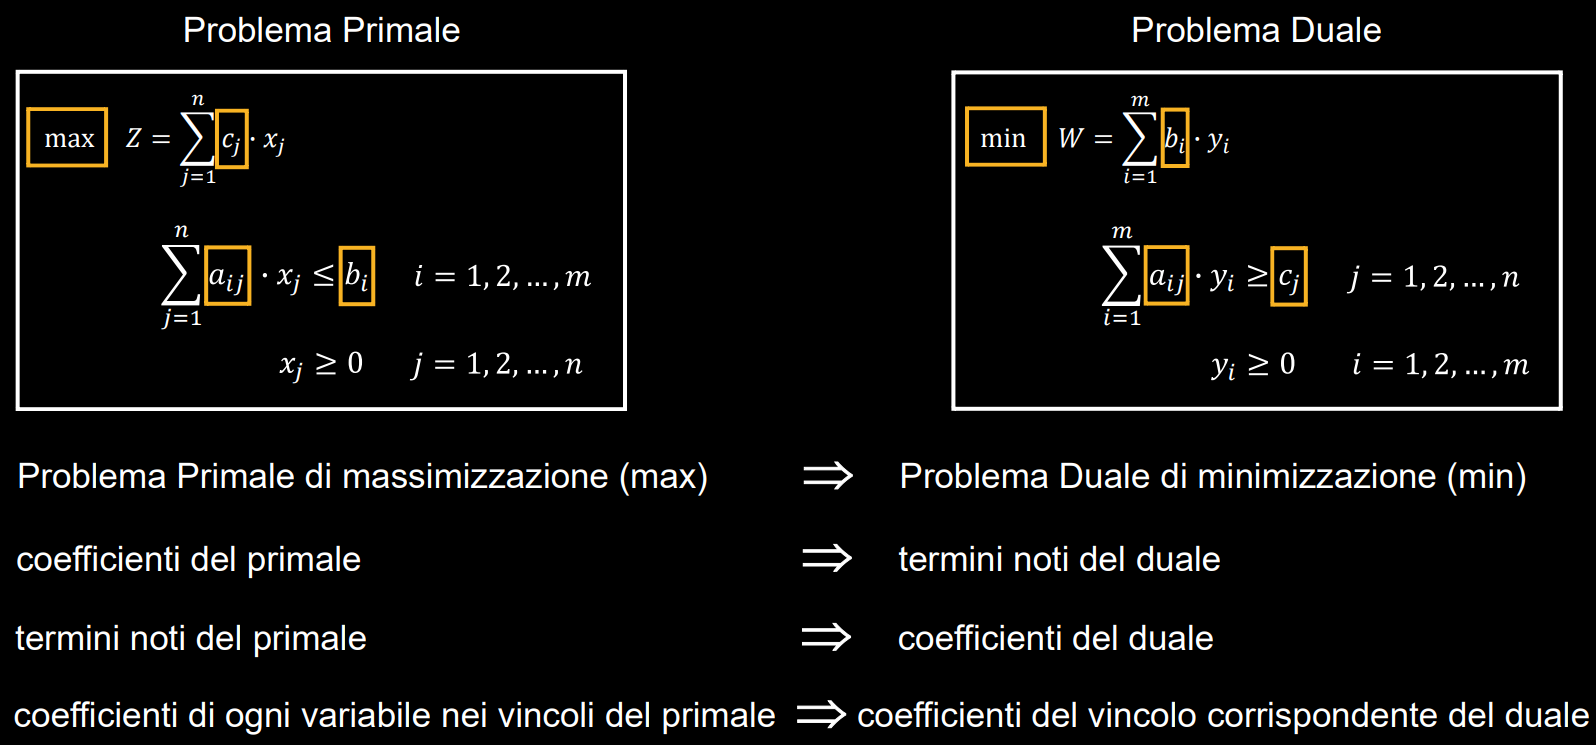
\includegraphics[width = 0.70\linewidth]{Images/44.png}
\end{center}
Tuttavia, nella realtà \textbf{il canale è sempre inaffidabile per definizione}: il protocollo IP è un protocollo "best-effort" e quindi non offre
garanzie sulla consegna, dovremo quindi \textbf{andare ad implementare dei meccanismi di trasporto che rendano la consegna affidabile}:
\begin{center}
    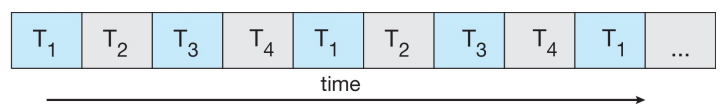
\includegraphics[width = 1\linewidth]{Images/45.png}
\end{center}
Abbiamo poi un ulteriore problema: il mittente e il destinatario \textbf{non conosco lo stato l'uno dell'altro} a meno che \textbf{non sia comunicato tramite messaggio}.
Consideriamo una \textbf{rete ideale}, cioè che non introduce:
\begin{itemize}
    \item Bit di errore
    \item Scarto di segmenti
    \item Segmenti fuori sequenza
\end{itemize}
Il livello di trasporto \textbf{allora non dovrà correggere nulla e il protocollo stesso sarà triviale}: il mittente invia i segmenti in sequenza (uno dopo l'altro) e il ricevente li riceve
senza nessun ulteriore controllo
\begin{center}
    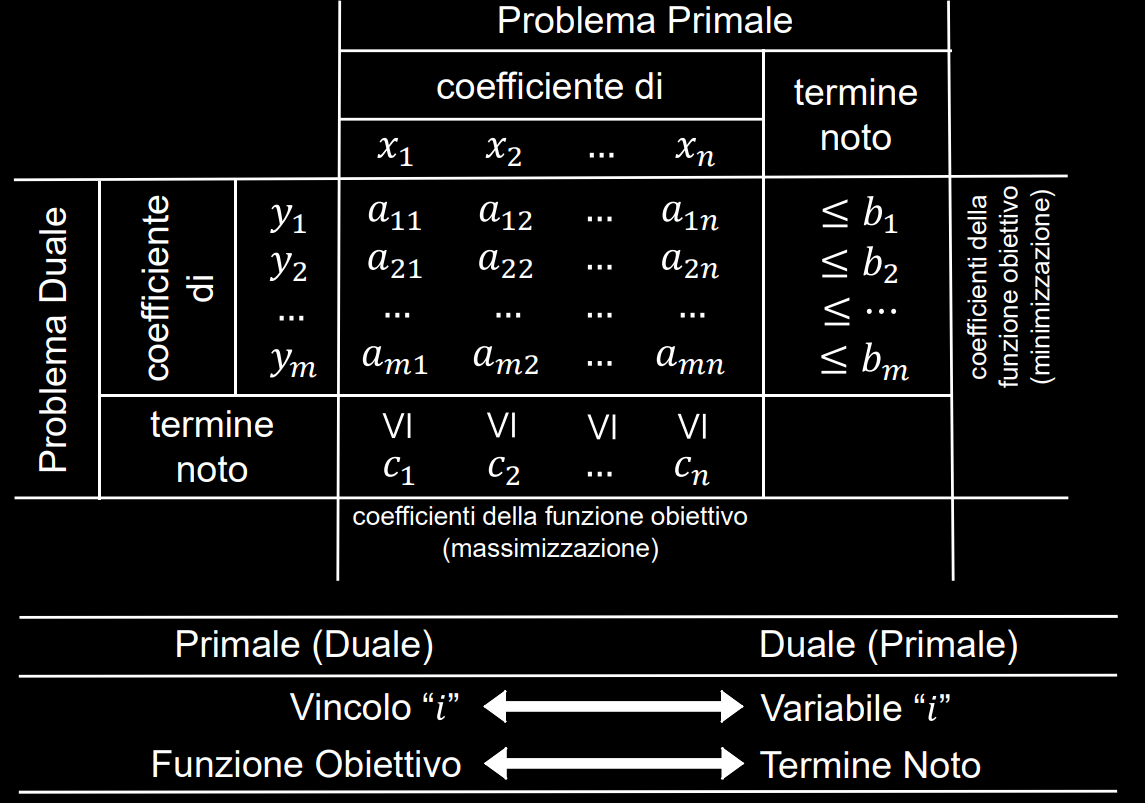
\includegraphics[width = 0.60\linewidth]{Images/46.png}
\end{center}
Sfortunatamente, le reti ideali non esistono. In una rete con errori, è possibile introdurre \textbf{riconoscimenti positivi} (ack) e \textbf{riconoscimenti negativi} (nack).
\begin{center}
    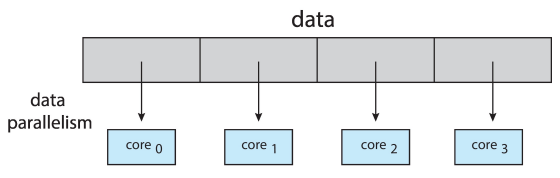
\includegraphics[width = 0.80\linewidth]{Images/47.png}
\end{center}
Un algoritmo di invio molto semplice allora potrà essere il seguente: \newline
\begin{algorithm}[H]
\DontPrintSemicolon
\eIf{ack} {
    $M_{i+1}$
} {
    \If{nack} {
        $M_i$
    }
    \If(\tcp*[h]{problema!}){?} {
        something
    }
}
\end{algorithm}
\noindent
Se la rete è \textbf{soggetta ad errori} anche \textbf{gli ack possono essere soggetti ad errori}, quindi stiamo ipotizzando, con questo algoritmo, che \textbf{la perdita o la corruzione di ack non avvenga}, cosa
che in realtà può accadere nelle reti reali. Un modo per mitigare questo problema è \textbf{ritrasmettere il messaggio se l'ack è corrotto}.
Tuttavia, neanche questo funziona! Non ho un meccanismo per capire se \textbf{un messaggio è duplicato o meno}. Possiamo mitigare ulteriormente questo problema nel seguente modo:
se i \textbf{segmenti sono numerati con un numero di sequenza nell'intestazione}, non c'è il rischio di non sapere se un messaggio è duplicato o meno
\begin{center}
    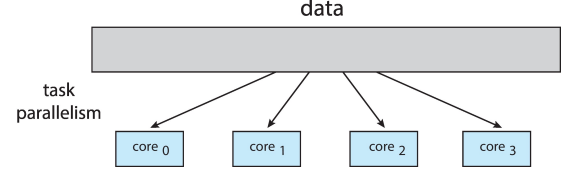
\includegraphics[width = 0.80\linewidth]{Images/48.png}
\end{center}
L'algoritmo di invio allora diventa: \newline
\begin{algorithm}[H]
\DontPrintSemicolon
\eIf{ack} {
    $M_{i+1}$
} {
    $M_i$ \tcp*[h]{è stato ricevuto un nack}
}
\end{algorithm}
\noindent
Un protocollo di questo tipo \textbf{funzionerebbe in una rete che introduce errori}. Sfortunatamente, le reti non solo introducono errori ma \textbf{anche perdite di pacchetti!}.
Prima di passare a definire un protocollo resistente anche alle perdite, parliamo di \textbf{efficienza di un protocollo}: quando si definisce un nuovo protocollo, si deve cercare di limitare
\textbf{il numero di messaggi diversi possibili in esso}, quindi se oltre a numerare i segmenti \textbf{numeriamo anche gli ack}
\begin{center}
    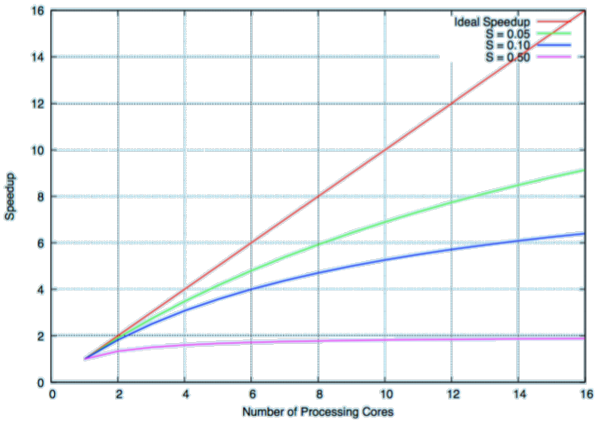
\includegraphics[width = 0.80\linewidth]{Images/49.png}
\end{center}
allora dovrò inserire una \textbf{regola aggiuntiva} che indica che, se non si è ricevuto il messaggio atteso, al posto di inviare un ack con numero di sequenza $i$ dovrò
inviare un ack con numero di sequenza $i-1$. L'algoritmo quindi diventa: \newline
\begin{algorithm}[H]
    \DontPrintSemicolon
    \eIf{ack} {
        $M_{i+1}$
    } {
        $M_i$ \tcp*[h]{è stato ricevuto un $ack_i$}
    }
    \end{algorithm}
\noindent
quindi, si andrà a ritrasmettere un messaggio se \textbf{si riceve un ack duplicato}.
Per rendere il protocollo resistente alle \textbf{perdite}: quando ho una perdita, può capitare che \textbf{il pacchetto inviato sia stato perso}
oppure che \textbf{l'ack vada perso}; allora viene introdotto \textbf{un timer}:
\begin{center}
    \includegraphics[width = 1\linewidth]{Images/50.png}
\end{center}
nel momento in cui \textbf{il timer scade} e non ho ancora ricevuto un ack, \textbf{rinvio lo stesso messaggio}. L'algoritmo di invio diventerà: \newline
\begin{algorithm}[H]
    \DontPrintSemicolon
    \eIf{$s+T$ is reached} {
        $M_i$\;
        set($s+T$) + $T$
    } {
        \eIf(\tcp*[h]{$s+T$ non è stato ancora raggiunto ($r$)}){$ack_i$} {
            $M_{i+1}$\;
            set($r+T$)
        } {
            $M_i$\;
            set($r+T$)
        }
    }
\end{algorithm}
\noindent
Questo tipo di implementazione è la più sofistica di quelli che vengono detti \textbf{protocolli stop-and-wait}.
Un protocollo stop-and-wait \textbf{funziona in una rete reale}. Tuttavia, vi sono delle problematiche:
\begin{itemize}
    \item L'impostazione della lunghezza del timer è un problema complesso
    \item Un timer \textbf{troppo corto} potrebbe causare \textbf{ritrasmissioni inutili}: nell'esempio fatto sopra, ci potrebbero essere lunghe sequenze di \textbf{ritrasmissioni inutili}
    \item Un timer \textbf{troppo lungo} ferma per troppo tempo la trasmissione in caso di perdita
\end{itemize}
\begin{center}
    \includegraphics[width = 0.25\linewidth]{Images/51.png}
\end{center}
Dovrò quindi avere un timer almeno lungo quanto il periodo di tempo che intercorre tra la trasmissione del messaggio e il ricevimento di un ack, questo valore
prende il nome di \textbf{Round-Trip Time} (RTT); il problema quindi passa al cercare di fare una stima accurata del RTT.
La problematica principale di un protocollo stop-and-wait è la seguente: supponiamo di essere nel caso in cui il \textbf{ritardo di trasmissione} non è più trascurabile
\begin{center}
    \includegraphics[width = 0.40\linewidth]{Images/52.png}
\end{center}
i parallelogrammi sopra rappresentano il ritardo di trasmissione, il quale vale $L/R$. Assumiamo, per semplicità, che gli ack
abbiano un ritardo di trasmissione trascurabile. Se siamo in un protocollo stop-and-wait, in questo caso esso è \textbf{altamente inefficiente}. Una
misura dell'efficienza del protocollo è la \textbf{utilità} (utility), la quale si calcola nel seguente modo:
$$U = \frac{\frac{L}{R}}{RTT + \frac{L}{R}}$$
questa misura indica \textbf{quanto tempo (da trasformare in percentuale) dedico effettivamente alla comunicazione}.
\subsubsection{Protocolli a finestra scorrevole}
\begin{center}
    \includegraphics[width = 0.30\linewidth]{Images/53.png}
\end{center}
Per risolvere il problema della \textbf{bassa utilità di stop-and-wait} sono stati pensati dei protocolli detti \textbf{a finestra scorrevole}
Questi protocolli permettono di trasferire fino a $W$ segmenti prima di \textbf{aspettare di ricevere gli ack dei vari segmenti inviati} (in questo caso si dice che la finestra si chiude).
Ciò significa che, una volta ricevuto l'ack del primo segmento \textbf{posso far scorrere la finestra e trasmettere il segmento $W$} e così via se non si hanno perdite. L'utilizzo del canale è quindi
molto più alto di stop-and-wait. La condizione per il quale c'è una condizione di \textbf{trasmissione continua} sul canale è che la finestra non si chiuda prima dell'arrivo del primo ack, cioè deve valere
la seguente condizione:
$$W \cdot \frac{L}{R} \geq RTT + \frac{L}{R}$$
invertendo la formula, posso quindi scoprire quanto deve essere grande la finestra per garantire una trasmissione continua:
$$W \geq \frac{RTT \cdot R}{L} + 1$$
C'è quindi da chiedersi \textbf{cosa deve essere ritrasmesso quando un segmento viene perso}.
Immaginiamo quindi di avere una finestra abbastanza ampia da non dover preoccuparci delle problematiche viste prima.
La prima possibilità è il protocollo \textbf{Go-Back-N}: la trasmissione va avanti e la finestra scorre \textbf{dopo ogni ack ricevuto}.
Se $s+T$ viene raggiunto, verranno ritrasmessi \textbf{tutti i segmenti a partire da quello che ha fatto scattare il timeout}
\begin{center}
    \includegraphics[width = 0.40\linewidth]{Images/54.png}
\end{center}
Il ricevitore, quando si accorge di aver ricevuto un segmento fuori sequenza, \textbf{scarta i segmenti fuori sequenza} e manda degli ack che "puntano" al primo segmento non ancora
ricevuto. Dal punto di vista del trasmettitore, appena inviato un segmento viene fatto partire un timer: se il timer scade, allora \textbf{ricomincerà a trasmettere tutti i segmenti a partire da quello per il quale il timer è scaduto}.
Tuttavia, questo protocollo non è particolarmente efficiente, perché \textbf{vado a scartare segmenti solo per poi riceverli di nuovo}, tuttavia questa implementazione \textbf{semplifica molto certi aspetti della trasmissione}: con questo protocollo
\textbf{non richiede buffer al destinatario}, poiché ogni segmento viene ricevuto in sequenza. Un'altra cosa importante di questo protocollo è il fatto che gli \textbf{ack sono comulativi}: per come è fatto il protocollo, i dati vengono
consegnati al livello applicativo \textbf{solo se sono in sequenza}; ciò significa che se io perdo un ack e successivamente l'ack per il segmento successivo \textbf{viene ricevuto correttamente}, allora posso essere sicuro che anche i segmenti successivi
siano stati trasmessi e ricevuti correttamente; cioè \textbf{gli ack dei segmenti successivi certificano la ricezione dei precedenti}. Ultimo dettaglio implementativo è che in questo protocollo \textbf{basta un solo timer per tutta la comunicazione}: viene fatto
ripartire dopo ogni ack ricevuto e si riferisce sempre al più vecchio segmento senza ack. \newline
Seconda possibilità è il protocollo \textbf{Selective Repeat}:
\begin{center}
    \includegraphics[width = 0.40\linewidth]{Images/55.png}
\end{center}
in questo protocollo, quando un segmento viene perso e il timer scatta per quel segmento, allora \textbf{viene ritrasmesso solo quel segmento} e non vengono
scartati gli altri segmenti. Chiaramente, in questo protocollo \textbf{ha la possibilità di avere segmenti fuori sequenza} e quindi ha bisogno di un buffer al
ricevitore per permettere il riordino dei segmenti prima di passarli al livello applicativo. Altra complicazione è che in questo protocollo gli ack sono \textbf{individuali}
e certificano solamente l'avvenuta ricezione di un segmento. Infine, \textbf{ogni segmento ha bisogno di un timer} per capire se esso è stato perso o meno.
Prima di continuare, facciamo un'osservazione: Go-Back-N e Selective repeat sono due esempi accademici l'uno opposto dell'altro. Nella realtà, si utilizzano \textbf{protocolli ibridi}
che utilizzano entrambi a seconda della situazione attuale della rete. TCP, infatti, è una soluzione ibrida tra questi due.
\subsection{Transmission Control Protocol (TCP)}
Transmission Control Protocol è un protocollo di trasporto \textbf{punto a punto}: vi è un singolo ricevitore e un singolo mittente che comunicano fra loro.
È un protocollo \textbf{affidabile}, che consegna i segmenti in ordine tramite uno \textbf{stream di byte}: in TCP quindi si fa riferimento ai \textbf{byte}, NON ai segmenti.
Non si hanno quindi \textbf{limiti del messaggio}, ciò che si va a fare è \textbf{contare i byte di dati all'interno del byte stream}; in ogni caso però i dati vengono inseriti nel
payload di un segmento e ogni singolo segmento può avere un payload di una certa dimensione massima, che prende il nome di \textbf{Maximum Segment Size} (MSS).
La comunicazione di TCP è \textbf{full-duplex}: vi è un flusso dati \textbf{bidirezionale} sulla stessa connessione.
TCP è \textbf{robusto a perdite di ack} e adotta il principio degli \textbf{ack comulativi}; inoltre è un protocollo \textbf{a finestra scorrevole}: per andare a impostare correttamente
la finestra d'invio utilizza due meccanismi di \textbf{controllo della congestione e di controllo del flusso}. È infine un protocollo \textbf{connection-oriented}, è quindi necessaria una fase
di "handshaking" (scambio di messaggi di controllo) in cui i due comunicanti si mettono d'accordo sui \textbf{parametri della connessione}.
La struttura di un segmento TCP è la seguente:
\begin{center}
    \includegraphics[width = 1\linewidth]{Images/56.png}
\end{center}
Alcune considerazioni:
\begin{itemize}
    \item Il bit $A$ viene settato ad 1 solamente se il messaggio è un \textbf{ack}: in TCP quindi ho solo messaggi o ack
    \item Le opzioni riguardano più ambiti (es. andare a negoziare la grandezza di MSS), quindi la grandezza di un header TCP è variabile e viene indicata dal campo \textit{header len}
    \item I bit $C$ ed $E$ servono ad indicare lo stato di congestione se si adotta la \textbf{congestione esplicita} e sono, in caso, impostati ad 1 dai router
    \item I bit $U$ e $P$ sono stati standardizzati e, se impostati ad 1, indicano che è necessario trasmettere \textbf{subito certi bit del pacchetto, considerati ad altra priorità}. Per come si è diffuso TCP, questi due bit non vengono quasi mai utilizzati
\end{itemize}
\subsubsection{Numeri di sequenza e di ACK}
Come vengono gestiti i \textbf{numeri di sequenza} e gli \textbf{ack} in TCP? Il numero di sequenza indica il \textbf{numero del byte stream del primo byte del segmento} mentre l'ack
indica il \textbf{numero di sequenza del prossimo byte che ci si aspetta di ricevere}. Vediamo quindi un esempio per fissare le idee:
\begin{center}
    \includegraphics[width = 0.80\linewidth]{Images/57.png}
\end{center}
\subsubsection{RTT in TCP e timeout}
Come viene impostato il timer di timeout in TCP? Questo aspetto è fondamentale per \textbf{evitare i problemi visti precedentemente} (trasmissioni inutili e tempi di risposta troppo alti)
Come facciamo però a stimare RTT? Nelle reti, il RTT varia molto e repentinamente tra segmenti di tipo diverso; dobbiamo quindi definire un meccanismo per cercare di impostare, in maniera approssimata,
un timer il più corretto possibile. Come fa TCP a stimare RTT?
\begin{itemize}
    \item Chiamiamo $SampleRTT$ il RTT che si misura dalla trasmissione al ricevimento dell'ack per un segmento specifico ignorando le ritrasmissioni.
    \item $SampleRTT$ cambia molto e in maniera repentina tra segmenti, vogliamo quindi \textbf{catturarne il trend}, non il $SampleRTT$ specifico: per impostare quindi il timer mi baserò su una misura meno netta, che chiamiamo $EstimatedRTT$, piuttosto che sul $SampleRTT$ del segmento precedente
\end{itemize}
Quindi come calcoliamo $EstimatedRTT$? Dobbiamo usare una tecnica che prende il nome di \textbf{Exponential Weighted Moving Average} (EWMA):
divido l'asse del tempo in \textbf{tempi discreti}, quindi l'$EstimatedRTT$ che deve essere calcolato al tempo $t$ è
$$EstimatedRTT[t] = (1-\alpha)\cdot EstimatedRTT[t-1] + \alpha \cdot SampleRTT[t]$$
\begin{center}
    \includegraphics[width = 0.65\linewidth]{Images/58.png}
\end{center}
L'influenza che i vari campioni sul valore di $EstimatedRTT$ decade esponenzialmente man mano che vado avanti nel tempo.
Un valore tipico di $\alpha$ è $\alpha = 0.125$. Per impostare l'intervallo di Timeout, dobbiamo però dobbiamo anche considerare
che le oscillazioni del RTT possono essere molto elevate, quindi impostiamo l'intervallo per il segmento che deve essere inviato al tempo $t$ nel seguente modo:
$$TimeoutInterval[t] = EstimatedRTT[t] + 4*DevRTT[t]$$
con l'ultimo addendo che rappresenta un "margine di sicurezza" per evitare i problemi legati ad una finestra impostata erroneamente.
$DevRTT[t]$ è la \textbf{deviazione}, calcolata tramite la tecnica EWMA, di $SampleRTT$ da $EstimatedRTT$ e si calcola nel seguente modo:
$$DevRTT[t] = (1-\beta)\cdot DevRTT[t-1] + \beta \cdot |SampleRTT[t] - EstimatedRTT[t]|$$
tipicamente, $\beta = 0.25$
\subsubsection{Trasmettiore TCP}
Ogni volta che si ricevono dati dallo strato applicativo, si effettuano le seguenti operazioni in un trasmettitore che usa TCP:\
\begin{itemize}
    \item Si crea un segmento con un numero di sequenza, il quale è definito come il primo byte del segmento all'interno del byte stream
    \item Viene fatto partire il \textbf{timer}: viene adottato un solo timer ed esso fa riferimento al più vecchio segmento per il quale non è stato ricevuto un ack. Viene impostato $TimeoutInterval$ utilizzano le formule viste sopra (per il primo pacchetto, $EstimatedRTT = SampleRTT$)
    \item Se \textbf{scatta il timeout}, ritrasmetto il segmento che lo ha causato e faccio ripartire il timer
    \item Una volta che viene ricevuto un ack, esso \textbf{risconta tutti i segmenti precedenti per i quali non sono ancora stati ricevuti degli ack}; si va ad aggiornare lo stato dei segmenti che prima si consideravano "in attesa di ack" e si fa ripartire il timer per i segmenti che non sono ancora stati riscontrati
\end{itemize}
\begin{center}
    \includegraphics[width = 0.75\linewidth]{Images/59.png}
\end{center}
\subsubsection{TCP fast retrasmit}
Il meccanismo \textbf{fast retransmit} fu introdotto dopo la pubblicazione delle specifiche di TCP. Esso fun introdotto per permettere di ritrasmettere in maniera rapida i segmenti persi
nel caso in cui la perdita di segmenti avvenga \textbf{in maniera sporadica} e non sia una condizione sistematica della rete.
\begin{center}
    \includegraphics[width = 0.85\linewidth]{Images/60.png}
\end{center}
Come funziona? Quando un segmento viene perso, \textbf{viene ritrasmesso dal ricevitore l'ack per l'ultimo segmento in ordine ricevuto}. Una volta che il trasmettitore riceve \textbf{3 ack duplicati} (senza contare il primo ack ricevuto, il quale riscontrava solamente la ricezione del segmento)
allora fast retransmit permette la \textbf{ritrasmissione del segmento con il più piccolo numero di sequenza non ancora riscontrato} anche se il timeout non è ancora scattato.
\subsubsection{TCP connection management e 3-way handshake}
\begin{center}
    \includegraphics[width = 0.95\linewidth]{Images/61.png}
\end{center}
Prima di iniziare a trasmettere, mittente e destinatario devono essere \textbf{d'accordo sullo stabilire una connessione e su quali parametri stabilire per essa}.
Infatti, alcuni parametri della connessione devono essere negoziati tra mittente e destinatario \textbf{prima} della trasmissione; questo viene effettuato attraverso 
\textbf{l'handshake}. TCP usa un \textbf{handshake a 3 vie}:
\begin{center}
    \includegraphics[width = 0.85\linewidth]{Images/62.png}
\end{center}
Le risorse vengono allocate \textbf{una volta ricevuto il messaggio di SYN} per il server e \textbf{una volta ricevuto il messaggio di SYNACK} per il client.
Già nell'ultimo messaggio, inoltre, potrei avere \textbf{un payload di dati}. TCP inoltre permette di chiudere la connessione tramite una negoziazione tra client e server:
\begin{center}
    \includegraphics[width = 0.85\linewidth]{Images/63.png}
\end{center}
Nel primo caso, il client vuole terminare la connessione, quindi il server \textbf{riscontra la volontà del client}, \textbf{termina l'invio dei dati restanti} e infine \textbf{chiude la connessione}.
Nel secondo caso, invece, il client vuole terminare la connessione e il server la chiude subito poiché \textbf{non ha ulteriori dati da inviare al client}. Notare che \textbf{anche un server può fare richiesta di terminazione di una connessione}.
\newpage
\subsubsection{TCP flow control}
\begin{center}
    \includegraphics[width = 0.65\linewidth]{Images/64.png}
\end{center}
Per mezzo del controllo di flusso, si permette che \textbf{il ricevitore possa controllare la quantità di dati che il mittente può inviare} per evitare di essere \textbf{sopraffatto e di portare i propri buffer al buffer overflow} (e quindi una perdita di segmenti).
Come si controlla a livello di trasporto il tasso di arrivo?
\begin{center}
    \includegraphics[width = 0.45\linewidth]{Images/65.png}
\end{center}
Il buffer ha una determinata dimensione $RcvBuffer$ e ad un certo istante di tempo, il buffer avrà una certa quantita di dati al suo interno
e una certa quantità di spazio libero, che chiamiamo $rwnd$. Il ricevitore quindi invia come feedback al mittente (immettendolo nell'header dell'ack nel campo \textit{receive window})
$rwnd$, in modo che il trasmettitore la quantità massima di dati che esso può accettare prima di andare in buffer overflow.
La finestra di trasmissione $W$ \textbf{viene quindi limitata in base al valore di receive window che esso riceve dal ricevente}.
\subsubsection{Principi del controllo di congestione}
Il controllo di congestione \textbf{riguarda la rete}: ci sono troppe sorgenti che inviano troppi dati troppo velocemente e quindi la rete non è in grado di gestirli.
In questo caso, si avranno \textbf{ritardi e possibili perdite di pacchetti}. È quindi \textbf{molto diverso dal controllo di flusso}.
Nel momento in cui la congestione cresce, \textbf{si ha una crescita dei pacchetti persi in rete}; se si adotta quindi un protocollo affidabile come TCP, si andrà ad \textbf{aumentare il numero di pacchetti ritrasmessi}.
L'aumento di ritrasmissioni quindi andrà a peggiorare la situazione. In questa situazione, si avrà \textbf{un aumento del throughput}, che andrà vicino al 100\% della capacità operativa della rete, tuttavia \textbf{si avrà una riduzione del "goodput"} (la quantità di dati ricevuti effettivamente utili all'applicazione)c
cala drasticamente
\begin{center}
    \includegraphics[width = 0.65\linewidth]{Images/66.png}
\end{center}
Vogliamo quindi tornare ad una situazione dove \textbf{throughput e goodput sono sovrapposti}. Un possibile approccio è il \textbf{controllo di congestione end-to-end}:
\begin{center}
    \includegraphics[width = 0.65\linewidth]{Images/67.png}
\end{center}
in questo tipo di controllo di congestione, la rete non dà \textbf{nessun feedback esplicito} e lo stato della rete viene \textbf{inferito in base alle perdite e dai ritardi dei segmenti e degli ack che vengono ricevuti dai sistemi host}.
Questo tipo di approccio è quello adottato da TCP.
Un altro approccio, non frequentemente adottato, è quello del \textbf{controllo di congestione network-assisted}: in questo tipo di controllo di congestione,
i \textbf{router} hanno la capacità di fornire informazioni puntuali riguardante il loro \textbf{stato di congestione} (si può fare utilizzando i bit $C$ ed $E$ dell'header TCP).
\begin{center}
    \includegraphics[width = 0.65\linewidth]{Images/68.png}
\end{center}
\subsubsection{TCP congestion control}
L'approccio di TCP al controllo di congestione si dice del tipo \textbf{Additive Increase Multiplicative Decrease}: si parte da un tasso di invio dei byte
molto basso che \textbf{incrementerò gradualmente} (additive increase); prima o poi, avverrà una perdita poiché il \textbf{tasso di invio è diventato troppo elevato}, in questo caso
vado a \textbf{dimezzare il tasso di invio per evitare che ci siano altre perdite}:
\begin{center}
    \includegraphics[width = 0.85\linewidth]{Images/69.png}
\end{center}
Vediamo quindi le fasi di questo meccanismo:
\begin{enumerate}
    \item \textbf{Slow start}: il numero di segmenti trasmessi (MSS) ad ogni RTT viene limitato dalla \textbf{finestra di congestione} $cwnd$.
    Quando la connessione inizia, viene \textbf{fatto incrementare esponenzialmente} il tasso di invio fino alla prima perdita di un pacchetto:
    \begin{itemize}
        \item Inizialmente, $cwnd = 1$
        \item $cwnd$ viene \textbf{raddoppiata} ad ogni RTT; ciò viene fatto \textbf{incrementando RTT ad ogni ack ricevuto}
    \end{itemize}
    In breve, \textbf{si ha un inizio lento, tuttavia il tasso di invio aumenta esponenzialmente}
    \begin{center}
        \includegraphics[width = 0.35\linewidth]{Images/70.png}
    \end{center}
    \item \textbf{Congestion avoidance}: Quando la crescita da esponenziale deve diventare lineare? TCP indica che ciò deve avvenire quando \textbf{$cwnd$ arriva a metà del suo valore prima dell'ultimo timeout sperimentato}. Questo meccanismo
    si può implementare attraverso una variabile che prende il nome di $sstresh$ che, quando si verifica un evento di perdita, viene posta a \textbf{metà del valore che aveva $cwnd$ prima dell'evento di perdita}
    \begin{center}
        \includegraphics[width = 0.65\linewidth]{Images/71.png}
    \end{center}
    La primissima implementazione di TCP (\textbf{TCP tahoe}), poneva immediatamente $cwnd$ ad 1 in caso di evento di perdita.
    Una versione più recente di TCP detta \textbf{TCP Reno} adotta invece il meccanismo di \textbf{Fast Recovery}: se l'evento di perdita è stato causato da \textbf{3 ack duplicati} invece che da un evento di \textbf{timeout},
    invece di andare ad impostare $cwnd$ ad 1, essa viene impostata a $cwnd = sshtresh + 3 \cdot MSS$; in caso di timeout, invece, rimane il comportamento di TCP Tahoe
\end{enumerate}
La trasmissione in TCP viene quindi dominata \textbf{o dalla finestra di congestione ($cwnd$) o dalla finestra di ricezione ($rwnd$)}, cioè se domina il controllo di flusso oppure il controllo di congestione
\begin{center}
    \includegraphics[width = 0.55\linewidth]{Images/72.png}
\end{center}
Quindi la finestra di trasmissione è posta a $min\{cwnd, rwnd\}$ bytes; dopodiché si aspetta un RTT per gli ack e infine si inviano altri byte.
Quando $cwnd < rwnd$, il controllo di congestione è dominante rispetto al controllo di flusso.
Il trasmettitore TCP quindi andrà a limitare la propria trasmissione, quindi deve valere che
$$LastByteSent - LastByteAcked \leq min\{cwnd, rwnd\}$$
$cwnd$ è \textbf{dinamicamente aggiustata} in base alle condizioni di rete osservate (implementando il controllo di congestione TCP).
$rwnd$ è invece aggiustato basandosi \textbf{sul valore ricevuto dal ricevente} (implementando il controllo di flusso TCP).
\section{Livello di rete: Piano dati}
\begin{center}
    \includegraphics[width = 0.75\linewidth]{Images/73.png}
\end{center}
L'obbiettivo del livello di rete è trasportare i segmenti provenienti dal livello di trasporto dal \textbf{mittente} al \textbf{ricevente}.
\begin{itemize}
    \item \textbf{Mittente}: incapsula i segmenti in \textbf{datagrammi} che passerà al livello di collegamento
    \item \textbf{Ricevente}: Decapsula i segmenti dai datagrammi e li consegna al livello di trasporto
\end{itemize}
I protocolli del livello di rete sono presenti in \textbf{tutti i dispositivi capaci di connettersi ad internet}, cioè sono presenti sia negli host che nei router.
In particolare, i \textbf{router}:
\begin{itemize}
    \item Esaminano campi dell'intestazione dei datagrammi che passano attraverso di loro
    \item Muovono i datagrammi dalle porte di input alle porte di output corretta, in modo da trasferire i datagrammi lungo un cammino punto a punto (end-to-end) corretto tra il mittente e il destinatario
\end{itemize}
Due funzionalità chiave del livello di rete sono:
\begin{itemize}
    \item \textbf{Inoltro (forwarding)}: Muove i pacchetti dal collegamento in input del router all'appropriato collegamento in uscita dello stesso
    \item \textbf{Instradamento (routing)}: Determina la strada che un pacchetto deve intraprendere per raggiungere, dalla sorgente, la propria destinazione. Questo processo viene effettuato attraverso \textbf{algoritmi e protocolli di routing}
\end{itemize}
Il livello di rete è suddiviso in \textbf{due diversi "piani"}:
\begin{itemize}
    \item \textbf{Piano dati (Data plane)}: Ha valenza \textbf{locale} e riguarda le funzioni che vengono eseguite dai singoli router della rete per determinare l'interfaccia corretta verso quale inviare il pacchetto. Determina quindi COME un datagramma che arriva alle porte di input di un router debba essere inoltrato alle sue porte in uscita. Il piano dei dati, quindi, implementa \textbf{l'inoltro}.
    \item \textbf{Piano di controllo (Control plane)}: Ha valenza \textbf{su tutta la rete} (network-wide). Determina come un datagramma debba essere instradato tra i router, lungo un percorso end-to-end, dall'host sorgente all'host destinazione. Il piano di controllo, quindi, \textbf{implementa l'instradamento}.
    In realtà, il piano di controllo, nella sua accezione più generale possibile, non implementa solamente l'instradamento ma anche tutti i protocolli e tutti gli algoritmi \textbf{necessari a far funzionare la rete}. Esistono due differenti approcci di implementazione del piano di controllo:
    \begin{itemize}
        \item \textbf{Algoritmi di instradamento tradizionali}: Approccio distribuito, in cui il piano di controllo della rete (o una sua parte) viene implementato su ogni singolo dispositivo di rete. Ogni singolo router quindi \textbf{implementa il piano di controllo} 
        \item \textbf{Software Defined Networking (SDN)}: Il piano di controllo viene \textbf{centralizzato e implementato su server remoti} (anche in cloud). Si ha quindi un \textbf{controllore centralizzato} che ha una \textbf{visione globale} della rete e che prenderà le decisioni riguardanti l'instradamento dei pacchetti.
    \end{itemize}
    Questi appunti tratteranno solamente il primo approccio.
\end{itemize}
Nell'approccio tradizionale, ogni singolo router \textbf{ha un piano di controllo in cui vengono eseguiti gli algoritmi di routing}; si ha quindi uno \textbf{scambio di messaggi tra i vari router} per fare in modo di \textbf{popolare correttamente le proprie tabelle di inoltro}.
\begin{center}
    \includegraphics[width = 0.80\linewidth]{Images/74.png}
\end{center}
Nell'approccio SDN, il piano di controllo viene \textbf{centralizzato in dei server}, i quali eseguono il controllore remoto; il quale si
interfaccerà con i dati provenienti da ogni singolo router per \textbf{ottenere informazioni sulla rete} (es. informazioni topologiche), ottenendo
così una \textbf{visione del piano dei dati}. Conoscendo quindi tutte le informazioni necessarie su tutti i router della rete, il controller può prendere
decisioni riguardanti l'instradamento dei pacchetti, cioè \textbf{genererà le tabelle di inoltro}, le quali verranno inviate ai singoli router per poter effettuare le operazioni di inoltro.
\begin{center}
    \includegraphics[width = 0.80\linewidth]{Images/75.png}
\end{center}
\subsection{Modello di servizio dello strato di rete}
Qual è il modello di servizio che viene adottato per trasportare, a livello di rete, i datagrammi dalla sorgente al destinatario?
Per esempio, ci potrebbero essere varie tipologie di servizi che potrebbero essere offerti a... 
\begin{itemize}
    \item \textbf{Singoli datagrammi}: garanzia di consegna, garanzia di consegna con un ritardo massimo di 40ms ecc...
    \item \textbf{Flussi di datagrammi}: Garanzia di consegna in ordine, larghezza di banda minima ecc...
\end{itemize}
Tuttavia, a livello di rete, il modello di servizio adottato è di tipo \textbf{"best effort"}, quindi \textbf{non vi sono}:
\begin{itemize}
    \item Garanzie sulla consegna dei datagrammi al ricevente
    \item Garanzie sull'ordine di consegna
    \item Garanzie sulla larghezza di banda disponibile per il flusso lungo il percorso end-to-end
\end{itemize}
\begin{center}
    \includegraphics[width = 0.80\linewidth]{Images/76.png}
\end{center}
\subsection{Architettura di un router}
L'architettura generica di un router può essere visualizzata nel seguente modo:
essa prevede l'esistenza \textbf{di un certo numero di porte (o interfacce) in ingresso} e di un certo numero di \textbf{porte (o interfacce) in uscita}.
In realtà, ogni singola porta di un router può agire \textbf{sia come porta di ingresso, sia come porta di uscita}, tuttavia, a livello funzionale, è necessario
mantenere una distinzione fra le due. Tra le porte di ingresso e le porte in uscita si trova una \textbf{maglia di commutazione ad alta velocità} (high-speed switching fabric), il quale è una
\textbf{rete fisica}, solitamente implementata con circuiti integrati, che mette in comunicazione \textbf{ogni singola interfaccia di ingresso con ogni singola interfaccia in uscita}.
La switching fabric, tuttavia, \textbf{non ha un collegamento da ogni singola porta in ingresso ad ogni singola porta in uscita} (full mesh), poiché ciò risulterebbe in una complessità \textbf{molto elevata};
invece, l'implementazione di questa rete segue delle teorie che \textbf{permettono di andare a definire delle "reti di commutazione" all'interno della maglia}, le quali permettono di mettere in comunicazione le porte di ingresso con le porte di uscita
\textbf{mantenendo limitato il numero di collegamenti complessivi}.
Le reti di commutazione devono garantire \textbf{la possibilità di inviare pacchetti da un'interfaccia in ingresso ad un'interfaccia in uscita indipendentemente da ciò che sta accadendo sulle altre interfacce}.
Se una rete ha questa proprietà si dice che essa è \textbf{non bloccante}.
Il componente che permette l'esecuzione di tutte le operazioni di routing è il \textbf{processo di routing} (routing processor), il quale si trova nel \textbf{piano di controllo} del livello di rete.
\begin{center}
    \includegraphics[width = 0.80\linewidth]{Images/77.png}
\end{center}
Dall'immagine sopra, possiamo notare che \textbf{il piano dei dati e il piano di controllo operano su ordini di tempo molto diversi tra di loro}:
\begin{itemize}
    \item A livello di piano dati, viene effettuato lo \textbf{spostamento dei pacchetti dalle interfacce di ingresso a quelle di uscita}. Questa operazione deve essere effettuata \textbf{il più velocemente possibile}, vista anche la grande mole di pacchetti
    che si possono avere in un singolo router. L'ordine di tempo quindi, in questo contesto, è nell'ordine dei \textbf{nanosecondi}
    \item Le decisioni prese a livello di controllo, invece, possono anche essere applicate alla rete in un tempo nell'ordine dei \textbf{millisecondi}
\end{itemize}
Le \textbf{porte in ingresso} di un router hanno la seguente architettura:
\begin{center}
    \includegraphics[width = 1\linewidth]{Images/78.png}
\end{center}
analizziamola nel dettaglio
\begin{itemize}
    \item \textbf{Terminazione di linea} (line termination): È l'interfaccia verso il mondo esterno (es. porta Ethernet); si occupa di \textbf{ricevere i bit in ingresso}. Le funzionalità della terminazione di linea sono quindi
    relative al \textbf{livello fisico}
    \item \textbf{Protocollo del livello di collegamento}: Una volta ricevuti i bit del pacchetto, essi vengono passati al \textbf{livello di collegamento}, dove viene effettuato un protocollo a livello di collegamento per organizzare i bit in una \textbf{trama} (frame) e decapsulare il pacchetto in un \textbf{datagramma}
    \item \textbf{Lookup e inoltro}: Si utilizzano le informazioni contenute nei campi dell'intestazione del datagramma (ricevuto dallo strato precedente) per \textbf{interrogare la tabella di inoltro memorizzata nella memoria dell'interfaccia di input} (lookup) allo scopo di \textbf{trovare una corrispondenza} (match). 
    L'inoltro del pacchetto verso una porta di output avviene quindi in base alla corrispondenza trovata. Questa serie di azioni vengono dette \textbf{"match plus action"}.
    Quali sono però i campi dell'intestazione del datagramma che vengono utilizzati per prendere decisioni a livello di inoltro?
    Nel caso specifico di internet, viene utilizzato un approccio \textbf{basato sull'indirizzo IP di destinazione} (destination-based forwarding) contenuto nell'intestazione del datagramma;
    tuttavia, esistono anche altri tipi di meccanismi (es. \textbf{source-based forwarding}, dove viene preso in considerazione anche l'indirizzo IP sorgente).
\end{itemize}
Ogni singola porta in ingresso presenta \textbf{una coda}; ciò significa che si può avere una \textbf{situazione di accodamento nelle porte di ingresso di un router} quando il tasso di arrivo dei pacchetti è maggiore rispetto alla velocità con la quale lo switching fabric è in grado di smaltirli verso le porte in uscita.
La velocità di inoltro della switching fabric dei pacchetti sulle porte di ingresso verso le interfacce di output prende il nome di \textbf{switching rate}:
\begin{itemize}
    \item Viene spesso misurato come \textbf{multiplo del tasso di linea (line rate) $R$ della porta di input/output}, cioè della \textbf{velocità della porta}
    \item Se si hanno $N$ porte di ingresso/uscita (il numero coincide poiché ogni porta di input può diventare una porta di output e viceversa), allora è desiderabile uno switching rate di almeno $N \cdot R$, poiché esso garantisce un accodamento nelle porte di ingresso \textbf{trascurabile}.
\end{itemize}
\begin{center}
    \includegraphics[width = 0.70\linewidth]{Images/79.png}
\end{center}
Perché questo è fondamentale? Se si è nella condizione in cui lo switching rate è più basso di $N \cdot R$ (tasso di linea di tutte le porte di ingresso), allora si potrebbe avere 
\textbf{un accodamento molto elevato nelle porte di ingresso} e quindi avere delle perdite dovute ad un buffer overflow. In più, un ulteriore problema generato da un accodamento significativo nelle porte
di ingresso è il problema del \textbf{Head-of-the-line (HOL) blocking}: i datagrammi che si sono accodati nelle porte di ingresso del router \textbf{vengono bloccati dai datagrammi che si trovano davanti a loro nella coda}, i quali, al momento, non possono essere trasmessi verso la porta di output corretta.
Perché si può verificare questo fenomeno?Se si hanno due pacchetti, \textbf{provenienti da interfacce in ingresso differenti}, che devono essere inoltrati \textbf{verso la stessa porta in uscita}, allora questo
trasferimento non può avvenire in contemporanea per entrambi i pacchetti. Infatti, se provassi a trasmettere i due pacchetti insieme, essi finirebbero per \textbf{mischiarsi} (si avrebbe quindi una \textbf{collisione}) e quindi diventerebbero entrambi \textbf{inintelligibili}.
Quindi, uno dei due pacchetti dovrà \textbf{aspettare che la trasmissione dell'altro pacchetto si concluda} prima di essere trasmesso. 
\begin{center}
    \includegraphics[width = 0.901\linewidth]{Images/80.png}
\end{center}
Il problema dell'HOL-Blocking può \textbf{provocare la crescita indefinita del tempo di accodamento}; ragione per il quale è assolutamente necessario dimensionare lo switching fabric in maniera opportuna. \newline
Una \textbf{porta di output} di un router è invece strutturata come segue:
\begin{center}
    \includegraphics[width = 0.901\linewidth]{Images/81.png}
\end{center}
La struttura è pressoché identica a quella di una porta di ingresso; ovviamente, le operazioni effettuate all'interno della porta di uscita sono quelle di \textbf{incapsulamento del datagramma in una trama del livello di collegamento} e la
trasmissione in uscita del pacchetto. Anche in questo caso, le porta di output presentano un \textbf{buffer}, nei quali i pacchetti si accoderanno ogni qual volta il tasso di arrivo dei pacchetti dello switching fabric è più elevato del tasso di trasmissione
delle porte. Si potrebbero quindi avere, anche in questo caso, ritardi di accodamento e buffer overflow. \textbf{L'accodamento nelle porte di output è un problema fisiologico dei router} ed è quindi non eliminabile; tutta la trattazione dei ritardi di accodamento
vista fino ad ora era quindi riferita \textbf{ad un accodamento nelle porte di output, assumendo un accodamento in input trascurabile}.
Poiché l'accodamento nelle porte di output non è eliminabile, si rende necessario \textbf{capire come gestire e trasmettere in uscita i pacchetti si accodano nel buffer}.
In generale, \textbf{non è vero che, in generale, il primo pacchetto che arriva è il primo pacchetto che viene trasmesso} (politica FIFO); in realtà, i pacchetti possono avere \textbf{priorità di tipo differente}, quindi 
si rendono necessaire delle politiche che \textbf{regolino sia lo scarto preventivo dei pacchetti} sia \textbf{quali pacchetti verranno scelti per essere trasmessi in uscita}:
\begin{itemize}
    \item \textbf{Drop policy}: Al posto di far riempire la coda fino al punto di riempirla, quindi arrivare ad una situazione in cui ogni pacchetto successivo viene scartato per buffer overflow, tendenzialmente si tende a \textbf{scartare preventivamente dei pacchetti} quando il livello di occupazione della coda raggiunge una certa soglia.
    Tendenzialmente vengono scartati i pacchetti a più bassa priorità.
    \item \textbf{Discipline di scheduling}: Una volta che si hanno dei pacchetti accodati, quali sono quelli che \textbf{verranno trasmessi per primi?} Esistono delle politiche diverse (es. \textbf{Priority scheduling}: chi ha la più alta priorità).  
\end{itemize}
\subsection{Internet Protocol (IP)}
Il \textbf{protocollo IP} è un protocollo dello strato di rete che si occupa dell'indirizzamento dell'instradamento dei pacchetto; esso è \textbf{fondamentale per il funzionamento della rete internet}.
Il datagramma del protocollo IP ha la seguente struttura:
\begin{center}
    \includegraphics[width = 1\linewidth]{Images/82.png}
\end{center}
Vediamoli più in dettaglio:
\begin{itemize}
    \item \textbf{Version}: Ha lunghezza di 4 bit e riguarda la versione del protocollo utilizzata (es. IPv4, IPv6 [quest'ultimo, non oggetto del corso])
    \item \textbf{Header length}: Ha lunghezza di 4 bit e riporta la \textbf{lunghezza dell'header in byte}. Questo campo si rende necessario poiché il protocollo IP \textbf{prevede la presenza di eventuali opzioni}, le quali possono allungare la dimensione dell'intestazione.
    \item \textbf{Length}: Ha lunghezza di 16 bit e riporta la \textbf{lunghezza totale del datagramma in byte}. Ovviamente $\textrm{Length} - \textrm{Header length} = \textrm{Payload length}$. Poiché si hanno 16 bit per codificare la lunghezza del datagramma, allora la sua massima dimensione possibile
    sarà $2^{16} - 1 \approx 65.000$ byte; solitamente, però, la lunghezza di un datagramma IP è di $1500$ byte perché si tende a dimensionare un pacchetto in modo tale che sia \textbf{al più grande quanto la massima lunghezza supportata da una trama a livello di collegamento}.
    \item \textbf{Type of service}: Ha lunghezza 8 bit ed indica la \textbf{priorità del pacchetto}
    \item \textbf{Time to live (TTL)}: Ha lunghezza 8 bit e non è altro che un \textbf{contatore} che viene decrementato da ogni router che il pacchetto attraversa. Il massimo del TTL è $2^8 - 1 = 255$.
    Questo campo è necessario per evitare che un pacchetto mal indirizzato o finito in un loop della rete \textbf{rimanga per sempre presente al suo interno}.
    \item \textbf{Upper layer}: Ha lunghezza 8 bit e indicano quale \textbf{protocollo di trasporto sta venendo utilizzato per il payload di questo pacchetto}; questo campo serve per \textbf{effettuare le operazioni di multiplazione e demultiplazione a livello di rete}.
    \item \textbf{Fragmentation reassembly}: Questi 3 campi, rispettivamente di 16, 4 e 12 bit, venivano utilizzati per la \textbf{frammentazione}. IP prevede che, nel caso il datagramma sia di dimensioni maggiori rispetto alla massima dimensione gestita dal protocollo di collegamento, esso possa essere \textbf{frammentato in pacchetti di dimensioni più piccole}, che poi alla destinazione verranno \textbf{ricombinati nel datagramma originario}.
    Di fatto, la frammentazione non avviene quasi mai nelle reti moderne. La frammentazione di un datagramma introduce diversi problemi, come \textbf{la necessità di dover avere un buffer al destinatario} o il \textbf{dover ricostruire un datagramma da dei pacchetti arrivati fuori sequenza}.
    \item \textbf{Header checksum}: Ha lunghezza 16 bit e viene usato per \textbf{effettuare un controllo su eventuali errori sul solo header IP (NON SUL PAYLOAD)}.
    \item \textbf{Source IP address}: Ha lunghezza 32 bit e indica l'indirizzo IP di chi ha generato il datagramma
    \item \textbf{Destination IP address}: Ha lunghezza 32 bit e indica l'indirizzo IP di destinazione del datagramma
    \item \textbf{Options}: Questo campo ha lunghezza 32 bit e indica diverse opzioni del protocollo IP che possono essere attivate per la trasmissione (es. Registrare il percorso effettuato)
\end{itemize}

\subsubsection{Indirizzamento IP}
%52:56







\end{document}